\newpage
\chapter{Séparation des réplicons}\label{chap4b}

\lhead{\emph{Séparation des réplicons}}\label{parclassifrepl}

Les clusters de protéines obtenus sont ensuite utilisés pour caractériser les réplicons bactériens. L'objectif est de séparer les réplicons sur cette base et de voir si des regroupements spécifiques émergent. Les réplicons sont d'abord visualisés par des techniques de projection ou après transformation en graphe. Ensuite, ils sont clusterisés afin d'explorer plus spécifiquement les groupes formés et le positionnement des RECE par rapport aux autres réplicons.

\section{Jeux de données obtenues et notations}\label{parjeuxdedonnees}
    
\subsection{Classification taxonomique}

Les génomes bactériens sont organisés  selon leur classification taxonomique, la hiérarchie des différents rangs taxonomiques suivant la relation:
	\begin{equation}\label{eqtax}
	\text{Espèce} \subset \text{Genre} \subset \text{Famille} \subset \text{Ordre} \subset{Classe} \subset {Phylum} \subset \text{Domaine}
	\end{equation}
Un individu (souche) d'une espèce bactérienne est caractérisé par son génome $g$, constitué d’un ou plusieurs réplicons. Soit $G=\{g_{1},...,g_{|G|}\}$, l'ensemble des génomes bactériens. On peut définir un génome $g$ donné par l'ensemble des réplicons de différents types $r_{i}$ qui le constituent:
	\begin{equation}\label{eqindiv}
	g= \{r_{1},...,r_{|g|}\}
	\end{equation} 

\subsection{Description des réplicons}

On attribue aux réplicons le descripteur taxonomique de la bactérie qui les héberge. Ils possèdent de plus un type appartenant à l'ensemble $\{ \text{chromosome, plasmide, RECE} \} $ (``\textbf{chr}" est utilisé comme notation abrégée de “chromosome” dans les équations).
Les clusters d’homologues de protéines des STIG permettent de caractériser les réplicons. Soient une solution de clustering des protéines $Cl=\{C_{1},...,C_{|Cl|}\}$, et l'ensemble des réplicons $R=\{r_{1},...,r_{|R|}\}$. Un réplicon $r$ peut être décrit par l'ensemble des gènes codant des protéines qu'il porte et est  \textit{de facto} défini par un ensemble de protéines:
	\begin{equation}
	r=\{p_{1},...,p_{n}\}
	 \end{equation}
 Un clustering de $R$, tel que $f_{clustering}(R)=\Big\{\{r_{k_{1}1},...,r_{k_{1}i}\},...,\{r_{k_{x}1},...,r_{k_{x}j}\}\Big\}$, est noté $Kl$.\\
 Un réplicon $r$ est caractérisé par le vecteur $v^{r}$ défini par:
  	\begin{equation}\label{eqvr}
  	v^{r}=(N^{r}_{C_{1}},...,N^{r}_{C_{|Cl|}})
	\end{equation}
	où  $N^{r}_{C_{i}}=|r \cap C_{i}|$ est le nombre de protéines de $r$ dans $C_{i}$, un cluster de protéines homologues.\\	
L'ensemble $V^{R}$ des vecteurs $v^{r}$ pour les réplicons $r$ de $R$  alors défini par:
	\begin{equation}\label{eqV}
	V^{R}=\{v^{r_{1}},...,v^{r_{|R|}}\}
        \end{equation}		

\subsection{Groupes structuraux et taxonomiques}

Soit une classe $K$ de réplicons. On  définit le vecteur pondéré des réplicons de $K$ par:
	\begin{equation}
	\bar{v}^{K}=(\bar{N}^{K}_{C_{1}},...,\bar{N}^{K}_{C_{|Cl|}})
	\end{equation}
où $\bar{N}^{K}_{C_{i}}$ est défini par:
	\begin{equation}
	\bar{N}^{K}_{C_{i}}=\frac{1}{|K|}\sum_{r \in K}N^{r}_{C_{i}}
	\end{equation}
$\bar{v}^{K}$ est alors le centre de gravité de la classe $K$.\\
Les réplicons étant organisés par type et par groupe taxonomique, les notations suivantes sont introduites:
\begin{description} 
\item[$\bullet$] $R_{taxon}$ désigne l'ensemble des réplicons de $R$ dont l'hôte appartient au groupe taxonomique $taxon$. $V^{R_{taxon}}$ désigne, par extension, l'ensemble des vecteurs $v^{r}$ des réplicons $r$ de $R_{taxon}$. 
\item[$\bullet$] $R^{\{type\}}$ désigne l'ensemble des réplicons, $r \in R$, où $Type(r) \in \{type\}$ et où $Type(r)$ est la fonction renvoyant le type de $r$.
\item[$\bullet$]  Pour un réplicon $r$ donné, la fonction $Tax_{n\_tax}(r)$ renvoie la valeur du rang taxonomique considéré de $r$ avec \textit{n\_tax} appartenant à la relation \ref{eqtax}. Par exemple, $Tax_{phylum}(r)=\text{\textit{Protéobactéries}}$ ou $Tax_{class}(r)=\text{\textit{Beta-protéobactéries}}$.
\item[$\bullet$] $Kl_{n\_tax}^{R}=\{K_{1},...,K_{|Kl|}\}$ est  l'ensemble des classes $K_{i}$ de réplicons où $K_{i} \subset  R$  tel que:
	 $$\begin{dcases}
	   Tax_{n\_tax}(r_{x})=Tax_{n\_tax}(r_{y}) &  r_{x},r_{y} \in K_{i}\\
	   Tax_{n\_tax}(r_{x})\neq Tax_{n\_tax}(r_{z}) &  r_{z} \in K_{j,\; j\neq i}\\
	  \end{dcases}
	   $$ 
Par exemple, $Kl_{phylum}^{R}$ sera l'ensemble des réplicons de $R$ organisés en classes selon le phylum d'appartenance de leur hôte.
\end{description}
	    
L'ensemble $\bar{V}^{Kl_{n\_tax}^{R}}$ des $\bar{v}^{K_{i}}$  où $K_{i} \in Kl_{n\_tax}^{R}$ est alors défini par:
	    \begin{equation}
	    \bar{V}^{Kl_{n\_tax}^{R}}=\{\bar{v}^{K_{1}},...,\bar{v}^{K_{|Kl_{n\_tax}^{R}|}} \}
	    \end{equation}
On définit $\bar{V}^{R}_{n\_tax}$ comme l'ensemble des vecteurs de réplicons de $R$ normés selon \textit{n\_tax} et regroupés par $type$ tel que:
	     \begin{equation}\label{eqVnorm}
	     \bar{V}^{R}_{n\_tax}= \bar{V}^{Kl_{n\_tax}^{R^{ \{chr\} }}} \cup \bar{V}^{Kl_{n\_tax}^{R^{ \{plasmide\} }}} \cup \bar{V}^{Kl_{n\_tax}^{R^{ \{RECE\} }}}
	     \end{equation}
Par extension $\bar{V}^{R_{taxon}}_{n\_tax}$ désigne l'ensemble des vecteurs de réplicons de $R_{taxon}$ normés selon $n\_tax$ et regroupés par type.\\

Pour un ensemble $Kl_{n\_tax}^{R_{i}}$ donné avec $R_{i} \subset R$, et pour $K \in Kl_{n\_tax}^{R_{i}} $, si tous les réplicons de $K$ sont du même type, on peut annoter $K$ selon les valeurs de $Tax_{n\_tax}(r)$ et de $Type(r)$ où $r \in K$. De même que pour un réplicon, on peut alors définir $Tax_{n\_tax}(K)$ et $Type(K)$ tels que $Tax_{n\_tax}(K)=Tax_{n\_tax}(r)$ et $Type(K)=Type(r)$ pour $r \in K$. On définit $\bar{Kl}_{n\_tax}^{R_{i}}$, l'ensemble des couples (\textit{Type}, $Tax_{n\_tax}$) existant dans $R_{i}$ par:
	\begin{equation}
	\bar{Kl}_{n\_tax}^{R_{i}} =\Big\{ \{Type(K) , Tax_{n\_tax}(K)\} |\;K \in  Kl_{n\_tax}^{R_{i}}\Big\}
	\end{equation}
$\bar{Kl}_{n\_tax}$, l'ensemble des couples (\textit{Type}, $Tax_{n\_tax}$) existant dans R est alors défini par:
	\begin{equation}
	\bar{Kl}_{n\_tax}=\bar{Kl}_{n\_tax}^{R^{ \{chr\} }} \cup \bar{Kl}_{n\_tax}^{R^{ \{plasmide\} }} \cup \bar{Kl}_{n\_tax}^{R^{ \{RECE\} }} 
	\end{equation}
	
  \subsection{Dimension des données}    
Sur l'ensemble des 5125 réplicons considérés et sur les \textbf{267.497} homologues identifiés (358.624 homologues présumés diminués des 91.127 faux positifs) pour une granularité $gr$ de 4 pour TRIBE-MCL, \textbf{4928} réplicons codent au moins une protéine parmi les homologues. \textbf{6096} clusters de protéines sont formés et sont considérés comme authentiques (ils ne correspondent pas à de faux positifs).

\begin{table}[H]
 	\caption[Dimension des données utilisées]{Dimension des données utilisées.\\ $R$ est l'ensemble des réplicons ayant au moins une protéine homologue. $Cl$ est la solution de clustering obtenue pour un $gr$ de 4 après la procédure de \textit{cleaning}.} 
	\begin{center}
 	\begin{tabular}{c|c|c}
 	\textbf{Données} & \textbf{Matrice} & \textbf{Taille}\\
	\hline
	$R$ & - & 4928\\
	$Cl$ & - & 6096\\
	$V^{R}$ & $M^{V^{R}}$ & (4928,6096)\\
	$\bar{V}^{R}_{genre}$ & $M^{\bar{V}^{R}_{genre}}$ & (851,6096)\\
	$\bar{V}^{R}_{classe}$ & $M^{\bar{V}^{R}_{classe}}$ & (91,6096)\\
	$\bar{V}^{R}_{phylum}$ & $M^{\bar{V}^{R}_{phylum}}$ & (60,6096)\\
	\end{tabular}
	\end{center}
\end{table}
    
    
\section{Méthodes d'évaluation de la séparation des réplicons}
    
    L'évaluation des méthodes de clustering est fondée sur des critères internes et/ou externes. Dans le cas de critères externes, la difficulté est de choisir les classes de référence auxquelles les clusters obtenus seront comparés. Ici, les clusters de réplicons obtenus sont analysés des points de vue structural (selon le type de réplicons) et taxonomique. L'efficacité des différentes méthodes de visualisation des données peut être estimée visuellement en inspectant la capacité des méthodes à séparer les données selon les critères utilisés pour le clustering: taxonomie et type, ainsi qu'en utilisant une procédure de clustering sur les données projetées suivie de la mesure de critères externes.
   
\subsection{Critères de validation externe utilisés}		    
   La structure génomique des STIG chromosomiques et plasmidiques différant (Chapitre \ref{chap1a}), une étude des réplicons bactériens selon leurs STIG doit mener à une discrimination nette des chromosomes et plasmides en des catégories distinctes. On peut postuler que les gènes liés aux STIG font, dans leur ensemble, partie du \textbf{\textit{génome-cœur}} des chromosomes. Il en ressort deux prédictions quant à la classification des réplicons par leurs STIG: i) les génomes stables (\textit{i.e.}, chromosomes) des individus de la même espèce auront des STIG très proches, et ii) l'homologie inter-espèces des STIG chromosomiques est retrouvée pour des représentants d'espèces proches phylogéniquement. Au final, deux critères externes sont mesurés:
    \begin{description}
    \item[\textbullet] la séparation et l'homogénéité des clusters de réplicons selon leur type,
    \item[\textbullet] l'homogénéité des clusters de réplicons selon la classification taxonomique de leur hôte.
    \end{description}
La comparaison externe de deux clusterings s'effectuera sur la base des scores obtenus pour ces deux critères. Un clustering pertinent, décrivant les réalités génomiques, aura une grande probabilité de respecter ces deux critères. L'hypothèse sur le second critère ne concernera que les réplicons chromosomiques et aucune supposition n'est faite quant aux scores obtenus pour des clusters de plasmides.  
 \\
 Les données utilisés sont $V^{R}$ avec $R$, l'ensemble des 5125 réplicons. À cause de la disparité de représentation de certains genres bactériens (par exemple, \textit{Escherichia, Vibrio, Burkholderia...} sont représentés par de nombreuses espèces et/ou souches, alors qu'un seul génome d'une seule espèce de \textit{Paracoccus}, \textit{Asticaccaulis}, \textit{Sphaerobacter} n'est présente dans $V^{R}$), l'ensemble $\bar{V}^{R}_{genre}$ est utilisé au lieu de $V^{R}$ dans certains cas. $\bar{V}^{R}_{genre}$ permet d'étudier non plus les individus mais les genres bactériens. Pour chaque couple \{\textit{genre,type}\}, un \textbf{vecteur normé} est construit avec comme valeur de chaque variable la moyenne des valeurs pour les variables des réplicons identifiés par ce couple (éq. \ref{eqVnorm}). Pour un clustering de réplicons $Kl$ formé, différents ensembles de réplicons de référence  $Kl_{ref}$ sont alors formés selon le type des réplicons, la taxonomie des espèces hôtes des réplicons, et selon que les données sont normées ou pas (Table \ref{tabklref}). L'évaluation des solutions de clustering des réplicons se fera par comparaison avec cinq ensembles de référence (Table \ref{tabklref}). 

 \begin{table}[h]
	\caption{Ensembles des classes de référence $Kl_{ref}$ selon la séparation étudiée.} \label{tabklref}	
	\begin{center}
 	\begin{tabular}{c|c|c}
	\textbf{Séparation étudiée} & \textbf{Ensembles non normés} & \textbf{Ensembles normés}\\
	\hline
	&\\[-0.2cm]
	type des réplicons & $\{R^{\{plasmide\}}, R^{\{chr\}}\}$ & $\{\bar{Kl}^{R^{\{plasmide\}}}_{genre}, \bar{Kl}_{genre}^{R^{\{chr\}}}\}$\\
	phylum des chromosomes & $Kl_{phylum}^{chr}$ & $\{\bar{Kl}^{K}_{genre}|\;  K \in Kl_{phylum}^{chr}\}$\\
	phylum des plasmides & $Kl_{phylum}^{plasmide}$ & $\{\bar{Kl}^{K}_{genre}|\;  K \in Kl_{phylum}^{plasmide}\}$\\
	classe des chromosomes & $Kl_{classe}^{chr}$ & $\{\bar{Kl}^{K}_{genre}|\;  K \in Kl_{classe}^{chr}\}$\\
	classe des plasmides & $Kl_{classe}^{plasmide}$ & $\{\bar{Kl}^{K}_{genre}|\;  K \in Kl_{classe}^{plasmide}\}$\\
	\end{tabular}
	\end{center}
\end{table}   

    
\subsubsection{V-measure}     
	  La \textit{V-measure} \citep{Rosenberg2007} est la moyenne harmonique des deux indices \textit{homogeneity} et \textit{completeness}, qui traduisent, respectivement, les degrés d'homogénéité et d'exhaustivité des clusters (Chapitre \ref{chap2}).
	 Soient un ensemble d'observations $E=\{e_{1},...,e_{|E|}\}$, $Kl$ un clustering de $E$, et $Kl_{ref}$ un ensemble de classes de référence des observations de $E$. La \textit{V-measure} est définie par:
	 \begin{subequations}\label{eqvm}
	 \begin{align}
	 V-measure= 2. \frac{homogeneity.completeness}{homogeneity+completeness}
	 \end{align}	 	  
	  où les indices \textit{homogeneity} et \textit{completeness} sont définis par:
	  \begin{align}
	  homogeneity= 
	  \begin{dcases}
	  1 & \text{si } H(Kl|Kl_{ref})=0\\
	  1 - \frac{H(Kl|Kl_{ref})}{H(Kl)} &\text{sinon}\\
	  \end{dcases}\\
	   completeness= 
	  \begin{dcases}
	  1 & \text{si } H(Kl_{ref}|Kl)=0\\
	  1 - \frac{H(Kl_{ref}|Kl)}{H(Kl_{ref})} &\text{sinon}\\
	  \end{dcases}
	  \end{align}
	  avec $H(Kl)$, l'entropie de $Kl$, définie par:
	  \begin{align}\label{eqentrop}
	  H(Kl) = - \sum_{C \in Kl}\frac{|C|}{|E|}.log(\frac{|C|}{|E|})
	  \end{align}\label{condentrop}
	  et $H(Kl|Kl_{ref})$, l'entropie conditionnelle de $Kl$ sachant $Kl_{ref}$, telle que:
	  \begin{align}
	  H(Kl|Kl_{ref}) = - \sum_{C \in Kl}\sum_{K \in Kl_{ref}}\frac{|C \cap K|}{|E|}.log(\frac{|C \cap K|}{|K|})
	  \end{align}
	  \end{subequations}
	 Les indices \textit{homogeneity}, \textit{completeness} et \textit{V-measure} sont, respectivement, des analogues des indices de \textit{précision}, \textit{sensibilité} et \textit{F-measure} (éq. \ref{eqsensitive}). Cependant, de par leurs définitions et contrairement aux indices de la \textit{F-measure}, ils prennent en compte de façon plus cohérente la taille et l'hétérogénéité des clusters et présentent des meilleures performances dans l'évaluation de plusieurs clusterings \citep{Rosenberg2007}.  \textit{Homogeneity} et \textit{completeness} prennent leurs valeurs dans l'intervalle $[0,1]$, une valeur de 1 indiquant de parfaites homogénéité et exhaustivité de $Kl$ par rapport à $Kl_{ref}$.\\
	  %L'entropie des équations \ref{eqentrop} et \ref{eqentrop} est similaire au critère introduit par Zhao \textit{et. al} \citep{zhao2001criterion}.
Dans les évaluations des clusters des réplicons, seule l'\textit{homogeneity} est vraiment discriminante. La \textit{completeness} est un indicateur du niveau auquel des classes différentes sont réparties dans des clusters distincts.
    
\subsection{Critères de validation interne}
\subsubsection{Coefficient silhouette}
	Dans un premier temps, nous avons mesuré les qualités intrinsèques des clusterings obtenus par des critères de performance classiques comparant les distances des observations intra-clusters et inter-clusters. Le \textbf{coefficient silhouette} (éq. \ref{eqsilhouette}) a d'abord été utilisé afin de mesurer l'enchevêtrement des clusters obtenus, notre objectif étant qu'il soit minimisé. Les mesures obtenues par ce critère semblent cependant peu pertinentes compte tenu de la très grande dimensionalité des données, et en comparaison des critères externes utilisés qui permettent d'évaluer le pouvoir de séparation d'un clustering en se référant à des concepts biologiques plus “concrets” que les distances mesurées par ce coefficient.\\
	 
	
\subsubsection{Critère de stabilité} 
Nous avons ensuite utilisé un critère de robustesse, estimant la stabilité des clusters. Un cluster stable témoignera soit d'une réalité analytique par rapport aux données utilisées, soit de l'inflexibilité d'une méthode particulière de clustering envers un jeu de données particulier \citep{hennig2007cluster}. Le caractère instable d'un cluster reflètera toujours une probabilité d'existence faible de celui-ci qui alors ne devra pas être interprété \citep{hennig2007cluster}.
L'approche utilisée, inspirée de Hennig \citep{hennig2007cluster}, consiste, pour un clustering donné $Kl$, à effectuer des ré-échantillonages $Ech_{Kl}=\{Kl_{1},...,Kl_{n}\} $ pour évaluer la conservation des clusters $C$ de $Kl$ dans les différents $Kl_{i}$ de $Ech_{Kl}$.
\\
Soit un ensemble $E=\{e_{1},...,e_{|E|}\}$ d'observations, une procédure de clustering $f_{clustering}$, et un clustering $Kl$ de E tel que $f_{clustering}(E)=Kl$. On applique la procédure suivante:
	\\\\
	%\begin{subequation}
\begin{longtable}{@{\hspace{-0.2cm}}p{0.1\textwidth}@{\hspace{-0.1cm}}p{0.9\textwidth}}
	(1) & \textrm{Un Bootstrap sur $E$ de $n$ échantillons, $Ech_{E}=\{E_{1},...,E_{n}\}$, est réalisé à partir de tirages aléatoires avec remise sur $E$}\\
	(2) & Pour chaque échantillon $E_{i}$ de $Ech_{E}$, on calcule $f_{Cl}(E_{i})$. \textrm{On note $Ech_{Kl}=\{f_{Cl}(E_{i})|\;  E_{i} \in Ech_{E}\}$}\\
	(3) & Soient un cluster $C$ tel que $C \in Kl$, un clustering $Kl_{i}$ tel que $Kl_{i} \in Ech_{Kl}$, et un ensemble d'observations $E_{i}$ tel que $E_{i} \in Ech_{E}$. On définit $\bigtriangleup_{i}^{C}$, comme la valeur:
	     	\begin{equation}
	     	\bigtriangleup_{i}^{C}=
				\begin{dcases}
			 	max\{d_{Jaccard}(C,C_{i}^{ech})|\; C_{i}^{ech} \in Kl_{i} \} & \textrm{si } C \cap E_{i} \neq\emptyset\\
			 	-1 & \textrm{sinon}
	 			\end{dcases}
	     	\end{equation}\\
	(4) & Soit $V_{\bigtriangleup_{i}^{C}}$, les valeurs prises par $\bigtriangleup_{i}^{C}$. L'\textbf{estimateur de stabilité du cluster} $C$, $\bigtriangleup^{C}$, est défini par:
	     	\begin{equation}
			\label{eqestimstabC}
			\bigtriangleup^{C}=\frac{1}{|B_{C}|}\sum_{E_{i} \in Ech_{E},\;\bigtriangleup_{i}^{C}\neq-1 }\bigtriangleup_{i}^{C}
	     	\end{equation}\\
	    & avec:
	     $$
		B_{C}=\{ \bigtriangleup_{i}^{C}|\; \bigtriangleup_{i}^{C}\in V_{\bigtriangleup_{i}^{C}} \textrm{ et }  \bigtriangleup_{i}^{C}\neq -1 \}
		$$\\
	(5) & $\bigtriangleup^{Kl}$, l'\textbf{estimateur de stabilité du clustering} $Kl$, est alors défini par:\\
	     &	\begin{equation}\label{eqestimstaball}
				\begin{split}
				\bigtriangleup^{Kl}=\frac{|C|}{|E|}\sum_{C \in Kl}\bigtriangleup^{C}
				\end{split}
	     	\end{equation}\\
	(6) & Soit $Cm^{Kl_{i}}_{C}$, un cluster de $Kl_{i}$ tel que $\bigtriangleup_{i}^{C}\neq-1$ et que $d_{Jaccard}(C,Cm^{Kl_{i}}_{C})$ est minimale pour l'ensemble des clusters de $Kl_{i}$. Un \textbf{estimateur de stabilité d'une observation} $e$ pour $e \in C$, $\bigtriangleup^{e}$, est défini par:
	     	\begin{equation}\label{eqestimstabr}
				\bigtriangleup^{e}=\frac{|B^{e}_{C}|}{|B_{C}|}
	     	\end{equation}\\
	     & avec:
		$$
		B^{e}_{C}=\{e \in Cm^{Kl_{i}}_{C}|\; Kl_{i} \in Ref_{Kl}\}
		$$\\
\end{longtable}

L'indice $\bigtriangleup^{Kl}$ est la moyenne des $\bigtriangleup^{C}$ pondérée selon la taille des clusters de $Kl$, ce qui diffère de la procédure originale de Hennig. $\bigtriangleup^{Kl}$ permet de comparer des solutions de clustering en donnant plus de poids aux clusters de grande taille. Pour un cluster $C$ de $Kl$ et une observation $e$ de $C$, $\bigtriangleup^{e}$ permet d'évaluer la stabilité de $e$ dans $C$ en évaluant le nombre de fois que $e$ est retrouvé dans les clusters $Cm^{Kl_{i}}_{C}$ des $Kl_{i}$ de $Ech_{Kl}$.\\
$\bigtriangleup^{e}$, $\bigtriangleup^{C}$ et  $\bigtriangleup^{Kl}$  prennent leurs valeurs dans l'intervalle $[0,1]$. Une valeur de $\bigtriangleup^{C}$ inférieure à 0.5 indique un cluster “dissous“ et non interprétable, alors qu'une valeur supérieure à 0.75 indique un cluster stable.\citep{hennig2007cluster,Hennig2008}.\\
La méthode de Fang et Wang \citep{Fang2010}, produisant un indice de stabilité similaire, a aussi été employée pour la selection du choix du nombre de clusters à utiliser en \textit{input} de l'algorithme WARD (voir ci-après).

\subsection{Sélection de modèle}\label{modelselec}\label{modelselect}
\subsubsection{Critères}
\begin{description}
	\item[$\blacktriangleright$] Les choix des algorithmes de clustering, des méthodes de projections et des paramètres sont guidés par les scores d'\textit{homogeneity} obtenus pour la séparation de l'ensemble des réplicons selon leur type, et pour la séparation des chromosomes selon leur taxonomie (phylum et classe). De façon complémentaire, l'indice de stabilité $\bigtriangleup^{Kl}$ des clusterings obtenus est également pris en compte. 
	\item[$\blacktriangleright$] Pour estimer la capacité des algorithmes à produire des clusters uniques pour chaque unité taxonomique, l'indice de \textit{completeness} est aussi considéré pour les séparations des chromosomes en fonction de leur appartenance à un phylum et à une classe taxonomique. Idéalement, une partition des données produit des clusters stables séparant plasmides et chromosomes et où, pour les clusters de chromosomes, la taxonomie des espèces-hôte des réplicons est retrouvrée.
	\item[$\blacktriangleright$] Pour un algorithme donné, la sélection des paramètres est principalement effectuée en fonction des scores de stabilité $\bigtriangleup^{Kl}$ et de l'indice de stabilité de Fang et Wang \citep{Fang2010}. En particulier, lorsque le nombre de clusters $k$ doit être entré, la valeur de $k$ est fixée lorsque une augmentation de $k$ n'entraîne pas d'accroissement significatif des scores des indices de stabilité des clusterings obtenus. 
	\item[$\blacktriangleright$] Les indices $\bigtriangleup^{C}$ et $\bigtriangleup^{e}$ permettent d'évaluer la pertinence d'un cluster ou d'une observation à l'intérieur d'un cluster donné.
\end{description}

\subsubsection{Sélection de modèle pour les méthodes de projection}
	Dans un premier temps, les différentes représentations des données sont comparées visuellement en estimant leur efficacité à structurer les données selon le type de réplicon ou la taxonomie de l'espèce-hôte. Afin de calculer des indicateurs, les données obtenues par les projections, $f_{P}^{2}(V^{R})$, sont soumises à une même procédure de clustering WARD utilisant un nombre de clusters fixé à 50. Les scores d'\textit{homogeneity}, \textit{completeness}, \textit{V-measure} et de stabilité $\bigtriangleup^{Kl}$ sont ensuite calculés à partir de ces clusters et permettent d'obtenir des mesures chiffrées pour les différentes projections de données. Cependant, si les projections ne produisent pas les mêmes types de partition, l'identification des partitions nécessitera des procédures spécifiques à chaque projection, ce qui risque d'apporter des biais à l'analyse. Nous estimons néanmoins que cette méthodologie ``maison" permet de proposer une première classification de l'efficacité des différentes projections du jeu de données.

     
\section{Visualisation des données}\label{visualis}
    Cette étape vise à représenter spatialement l'organisation des réplicons selon leur contenu en gènes des STIG de façon interprétable et pertinente, et d'identifier le positionnement des RECE par rapport aux autres réplicons. Les études traditionnelles de génomique comparative ont souvent recours à des structures de type arbre pour représenter les liens entre différents éléments génétiques, les liens recherchés étant classiquement des liens phylogéniques et évolutifs. Ces approches ne sont pas appropriées pour représenter les relations entre réplicons pour plusieurs raisons. i) Compte tenu des diversités des réplicons et de leurs STIG, la comparaison de deux réplicons peut difficilement être transformée en distance évolutive. ii) Un modèle de descendance linéaire entre les réplicons est simpliste et ne prend pas en compte les phénomènes d'échanges latéraux à l’œuvre dans les génomes bactériens \citep{Bapteste2009,Doolittle2007}. iii) Des mosaïques de STIG caractérisent les réplicons bactériens (\textit{c.f.} Chapitre \ref{chap1a}). Étudier une famille donnée de gènes ou de protéines, par exemple, les ParA/ParB, n’est pas suffisant pour décrire la diversité des STIG existant au sein des réplicons, l'objectif sous-jacent étant précisément de rendre compte de cette diversité.\\
L'exploration des données a donc reposé sur deux approches méthodologiques de visualisation:
	  \begin{description}
	  \item[\textbullet] La projection des données dans un espace de dimension réduite, 2D ou 3D, interprétable visuellement.
	  \item[\textbullet] La transformation des données en graphe (bipartite) et sa visualisation par ``spatialisation".
	  \end{description}
	  

\subsection{Réduction de dimension des données par projection}
\subsubsection{Méthodes utilisées}
	   Quatre types de projection ont été étudiés pour réaliser la projection des ensembles $V^{R}$ et $\bar{V}^{R}_{genre}$ dans des espaces à deux dimensions (\ref{tabprojec}).
   	   
      \begin{longtable}{ @{\hspace{-2.2cm}} >{\bfseries}p{0.05\textwidth}|>{\small}p{1.0\textwidth} }
      \caption[Méthodes de projection utilisées]{Méthodes de projection utilisées dans l'analyse des données.}\\ \label{tabprojec}
      \textbf{ACP} & L'\textbf{A}nalyse en \textbf{C}omposantes \textbf{P}rincipales \citep{hotelling1933analysis} est une méthode statistique permettant d'exprimer les valeurs de $p$ variables corrélées tirées de $n$ observations en $q$ variables non-corrélées, de manière à ce que les $q$ variables soient des combinaisons linéaires des $p$ variables et qu'elles soient orthogonales entre elles selon une distance $d$. Les $q$ variables, ou \textit{composantes}, définissent un espace en $q$ dimensions ($q < p$) dans lequel sont projetées les observations. Les $q$ variables sont choisies pour que la variance entre observations soit maximisée (et donc que l'\textit{inertie} des observations par rapport aux $q$ composantes soit minimale \citep{duby2006analyse}). Le seul paramètre à choisir est  $q$, le nombre de dimensions, $d$ étant la distance Euclidienne.
\\[0.4cm]
      \textbf{MDS} & L'ensemble de procédures \textit{\textbf{M}ulti\textbf{D}imensional \textbf{S}caling} permet de positionner des observations dans un espace de dimension réduite \citep{izenman2008modern}. Un exemple classique de procédure MDS métrique, $f_{MDS}^{q}$, pour un ensemble d'observations dont les vecteurs associés sont rassemblés dans $V$, consiste à minimiser la quantité: 
      \begin{equation} 
      Stress=\sum_{i<j}  \Big(d_{euclidienne}(v_{i},v_{j}) - d(f_{MDS}^{q}(v_{i}),f_{MDS}^{q}(v_{j}))\Big)^{2}
      \end{equation}
      pour tout $v_{i}$ et tout $v_{j}$ de $V$, et où $d_{euclidienne}$ est la distance euclidienne. Cette quantité peut servir à valider la projection des données (typiquement $Stress<0.20$ \citep{izenman2008modern}). Les paramètres à choisir sont la distance $d$ utilisée pour comparer les observations et des paramètres propres à la méthode de convergence de $Stress$ vers un minimum (nombre d'itérations, d'instantiation...)
\\[0.4cm]
     \textbf{ISOMAP} & Cette procédure est une méthode de réduction non-linéaire ne conservant que localement les distances entre une observation et les autres \citep{tenenbaum1998mapping,tenenbaum2000global}. Pour une observation $o$ et une distance $d$ donnée, l'algorithme cherche les $k$ voisins $o_{k_{i}}$ de $o$ tels que les $d(o,o_{k_{i}})$ soient minimales. Ces distances sont alors conservées. Pour calculer la distance séparant $r$ d'une observation n'appartenant pas à ses $k$ plus proches voisins, la distance \textit{géodésique} correspondant au chemin le plus court dans le graphe formé par les $k$ plus proches voisins est alors utilisée. Ces distances estimées sont ensuite utilisées dans une procédure de type MDS. Les paramètres de l'algorithme ISOMAP sont la distance $d$ initialement utilisée (généralement la distance Euclidienne), le nombre de voisins $k$, et les paramètres liés à la procédure MDS.
\\[0.4cm]
      \textbf{SOM} & L'algorithme de \textit{\textbf{S}elf-\textbf{O}rganizing \textbf{M}ap} \citep{Kohonen1982} consiste à assimiler chaque observation $o$ et son vecteur associé $v_{o}$ à l'une des cellules d'un ensemble de cellules $D$ organisées en $q$ dimensions. Plus précisément, une cellule $c$ est représentée par un vecteur $v_{c}$ de même dimension que $v_{o}$ et est assimilée à $o$ si et seulement si $d(v_{o},v_{c})=min\{d(v_{o},v_{c})|\; c \in D\}$. Ce processus est itératif et les valeurs de $v_{c}$ sont modifiées à chaque itération pour tendre vers celles de $v_{o}$. Les coordonnées de $c$, $\{x_{1},...,x_{q}\}$ dans $D$, correspondent alors à $f_{SOM}^{q}(v_{o})$ si $o$ est assimilée à $c$ à la dernière itération \citep{izenman2008modern}. Les paramètres à choisir sont le nombre d'itérations, les dimensions de $D$ et la distance $d$ utilisée.
      \end{longtable}
      
      La projection par ACP a d'abord été utilisée mais n’a pas permis d’obtenir une structuration pertinente des réplicons (voir ci-après). D’autres méthodes ont alors été employées. La procédure MDS a été testée avec la distance \textit{cosine} (éq. \ref{eqcosine}) ainsi qu’avec la distance Euclidienne modifiée (éq. \ref{eqeuclidmodif}). L'algorithme SOM, utilisé dans des domaines d’étude variés, constitue une alternative originale aux méthodes de visualisation classiques. Nous avons également eu recours à l'algorithme ISOMAP qui a été créé spécialement pour prendre en compte la non-linéarité de certains jeux de données, ce qui justifie son choix dans l'analyse.

\subsubsection{Logiciels utilisés}
 \begin{description}
 \item[Scikit-learn] librairie de Machine learning de Python a été utilisée pour le calcul des projections par ACP, MDS et ISOMAP, et celui des indices de V-measure (\textit{homogeneity}, \textit{completeness} et \textit{V-measure}) et des clusters WARD.
 \item[Python] a été utilisé pour réaliser les nombreux workflows, préparer les données, et calculer les distances inter-observations. 
 \end{description}
           
\subsubsection{Paramètres des analyses}
     % \begin{small}
 \begin{description}
\item[$\blacktriangleright$] Les choix du nombre d'itérations et des dimensions des cellules de SOM ont suivi les recommandations pour cette méthode \citep{wendel2010formalizing}.
\item[$\blacktriangleright$] Pour l’algorithme MDS, le choix de la distance s’est porté sur la distance \textit{cosine} (éq. \ref{eqcosine}), qui produit des résultats significativement meilleurs que les distances euclidiennes. Les paramètres additionnels sont les paramètres par défaut. 
\item[$\blacktriangleright$] Le nombre de voisins d'ISOMAP ($k$ = 5) a été choisi en fonction des valeurs des indices d'\textit{homogeneity}.
\item[$\blacktriangleright$] Le nombre de clusters $k$ utilisés par l'algorithme WARD sur les projections $M^{V^{R}}_{P}$ et $M^{\bar{V}_{genre}^{R}}_{P}$ de, respectivement, $V^{R}$ et $\bar{V}_{genre}^{R}$ a été choisi sur la base des scores de l'indice de stabilité de Fang et Wang obtenus. Un unique $k$ est choisi pour des différentes projections $M^{V^{R}}_{P}$ pour une raison d'homogénéité.
 \end{description}
 
 \subsubsection{Projection de $V^{R}$ et de $\bar{V}_{genre}^{R}$}
   Les méthodes de projection par ACP et ISOMAP se sont révélées inefficaces pour la représentation des réplicons. On peut noter des scores particulièrement faibles des indices d'\textit{homogeneity} obtenus pour la structuration des chromosomes selon la classe ou le phylum de leur hôte par ces méthodes (Table \ref{tabscorevisu}). Ces méthodes sont globalement moins performantes, et très peu performantes à séparer les chromosomes selon l'appartenance de leur hôte à un groupe taxonomique.

\begin{table}[H]
     \caption[Évaluation des procédures de visualisation de l'ensemble des réplicons]{Évaluation des procédures de visualisation de l'ensemble $V^{R}$ des réplicons.}\label{tabscorevisu} 
      \begin{tabular}{@{\hspace{-1cm}\hspace{1cm}} p{0.3\textwidth}|l|c|c|c|c}
       & \textbf{Indice$^{a}$}  & \textbf{SOM}  & \textbf{MDS} &\textbf{PCA$^{d}$}  & \textbf{ISOMAP}\\
      \hline
      Paramètres$^{b}$ &  & $it$:60000 & $d$: \textit{cosine} &  & $k$:5 \\
      Nombre de clusters$^{c}$ & & 50 & 50 & 50 & 50 \\
      \hline
      \multirow{3}{*}{Type de réplicons} & \textit{homogeneity} & 0.84 & 0.85 & 0.79 & 0.71\\
      &\textit{completeness} & 0.18 & 0.18 & 0.25 & 0.19\\
      &\textit{V-measure} & 0.29 & 0.29 & 0.38 & 0.30\\
      \hline
      \multirow{3}{*}{Phylum des chromosomes} & \textit{homogeneity} & 0.83 & 0.78 & 0.66 & 0.70 \\
      &\textit{completeness} & 0.50 & 0.46 & 0.33 & 0.35\\
      &\textit{V-measure} & 0.62 & 0.58 & 0.44 & 0.47\\
      \hline
      \multirow{3}{*}{Classes des chromosomes} & \textit{homogeneity} & 0.85 & 0.78 & 0.68 & 0.73 \\
      &\textit{completeness} & 0.75 & 0.68 & 0.49 & 0.54\\
      &\textit{V-measure} & 0.80 & 0.72 & 0.57 & 0.62\\
      \hline
      \multirow{3}{*}{Phylum des plasmides} & \textit{homogeneity} & 0.65 & 0.41 & 0.05 & 0.20 \\
      &\textit{completeness} & 0.31 & 0.26 & 0.12 & 0.17\\
      &\textit{V-measure} & 0.42 & 0.36 & 0.07& 0.18\\
      \hline
      \multirow{3}{*}{Classes des plasmides} & \textit{homogeneity} & 0.62  & 0.41& 0.06 & 0.17\\
      &\textit{completeness} & 0.41 & 0.27 & 0.22 & 0.21\\
      &\textit{V-measure} & 0.50 & 0.33 & 0.10 & 0.19\\
      \hline
      \end{tabular}
      \vspace{0.5cm}
      \captionsetup{labelsep=space,justification=justified,singlelinecheck=off}
     \caption*{$^{a}$ \textit{V-measure} calculées selon l'éq. \ref{eqvm}. \\ $^{b}$ $it$, nombre d'itérations utilisées par SOM, $d$ distance utilisée par l'algorithme MDS et $k$, nombre de voisins considérés par l'algorithme ISOMAP \\ $^{c}$ nombre de clusters donnés en \textit{input} pour l'algorithme WARD. \\$^{d}$ variance expliquée par les 2 principales composantes: 16\% }
	\captionsetup{}	
	\end{table}
      		%\begin{adjustwidth}{-3cm}{-3cm}
 
La difficulté qu'a l'ACP à séparer chromosomes et plasmides peut provenir du fait qu’ils ne sont pas linéairement séparables. La non-linéarité résulte en partie de la très grande dimension des données. La distance euclidienne entre deux chromosomes proches (à un certain degré) peut être plus élevée que celle séparant deux plasmides n'ayant rien en commun (\textit{c.f.} Chapitre \ref{chap2} \S \ref{parclustperf}). De nombreux réplicons, dont l'ensemble des plasmides, sont agrégés en un unique groupe (Figures \ref{figPCA} et \ref{figISOMAP}), témoignant de la difficulté des méthodes ACP et ISOMAP à structurer des observations qui ne possèdent que quelques attributs non nuls.
	  
\begin{figure}[H]
	\begin{minipage}{0.50\textwidth}
	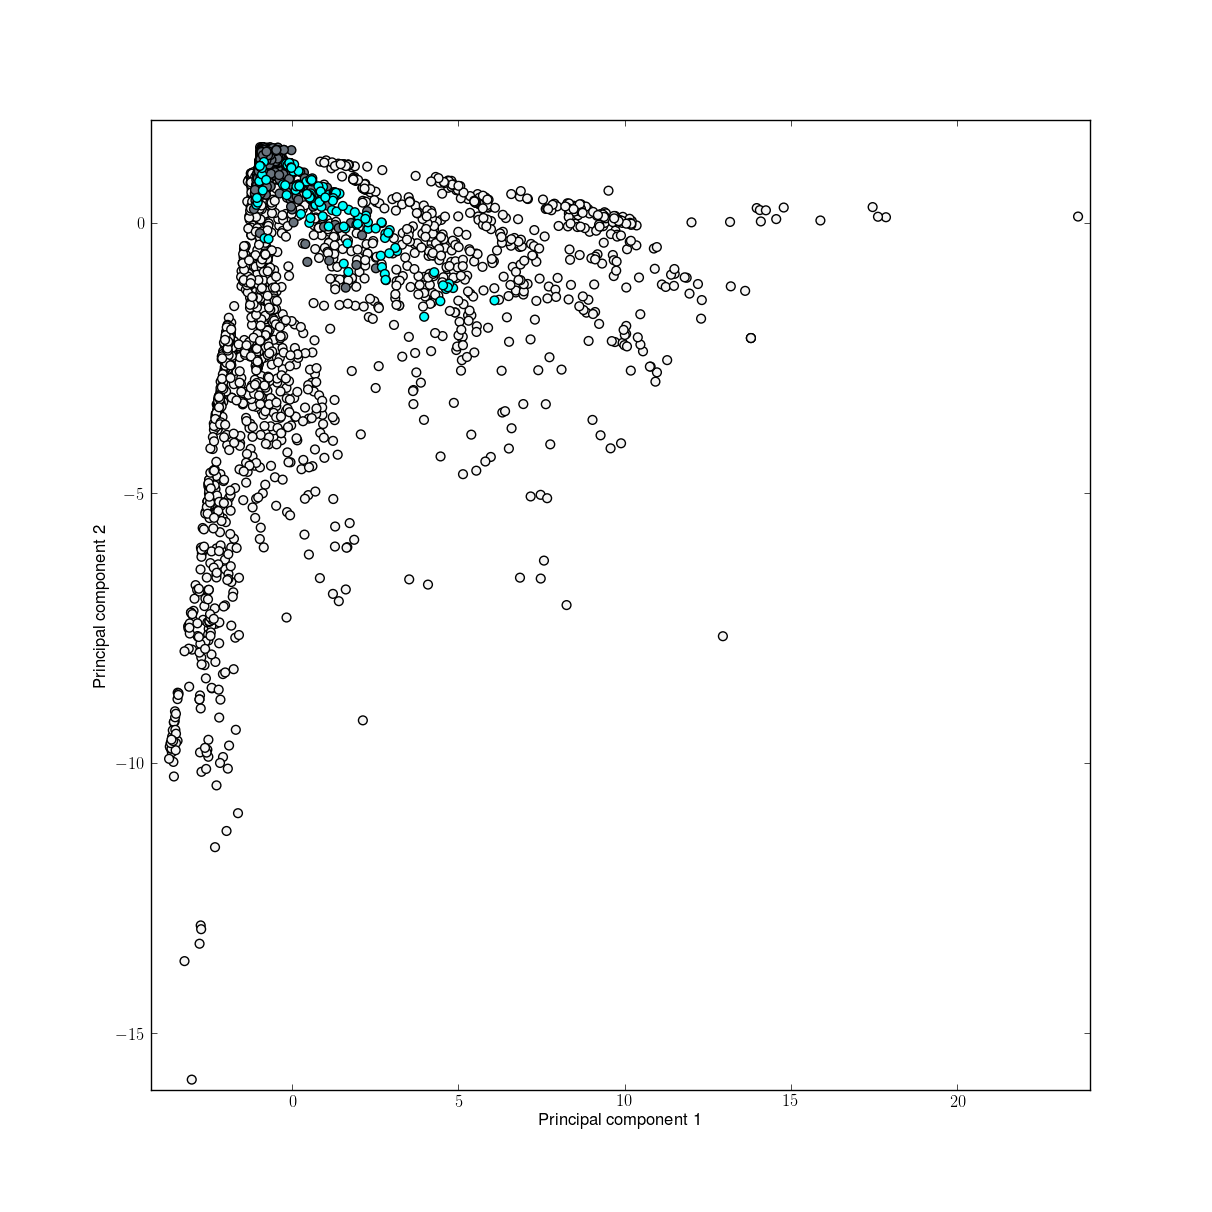
\includegraphics[trim=3cm 3cm 2cm 2cm,clip, width=\textwidth]{./img/pca_visu.png}
	\subcaption{$ACP$}\label{figPCA}
	\end{minipage}
	\begin{minipage}{0.50\textwidth}
	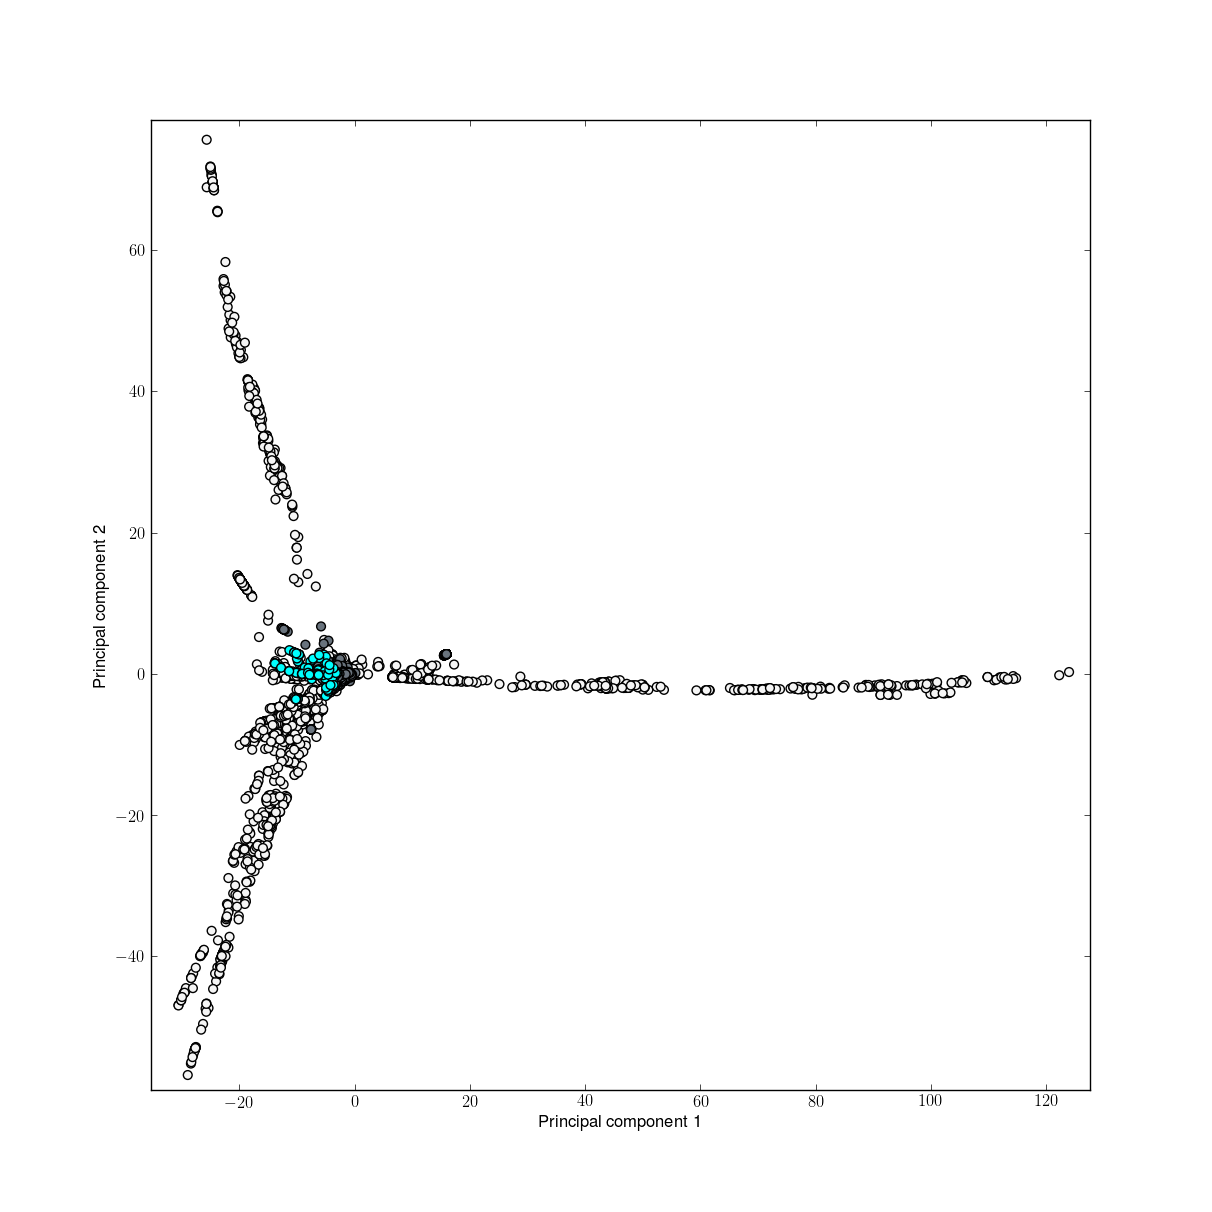
\includegraphics[trim=3cm 3cm 2cm 2cm,clip, width=\textwidth]{./img/ISOMAP.png}
	\subcaption{$ISOMAP$}\label{figISOMAP}
	\end{minipage}
	\\
	\begin{minipage}{0.50\textwidth}
	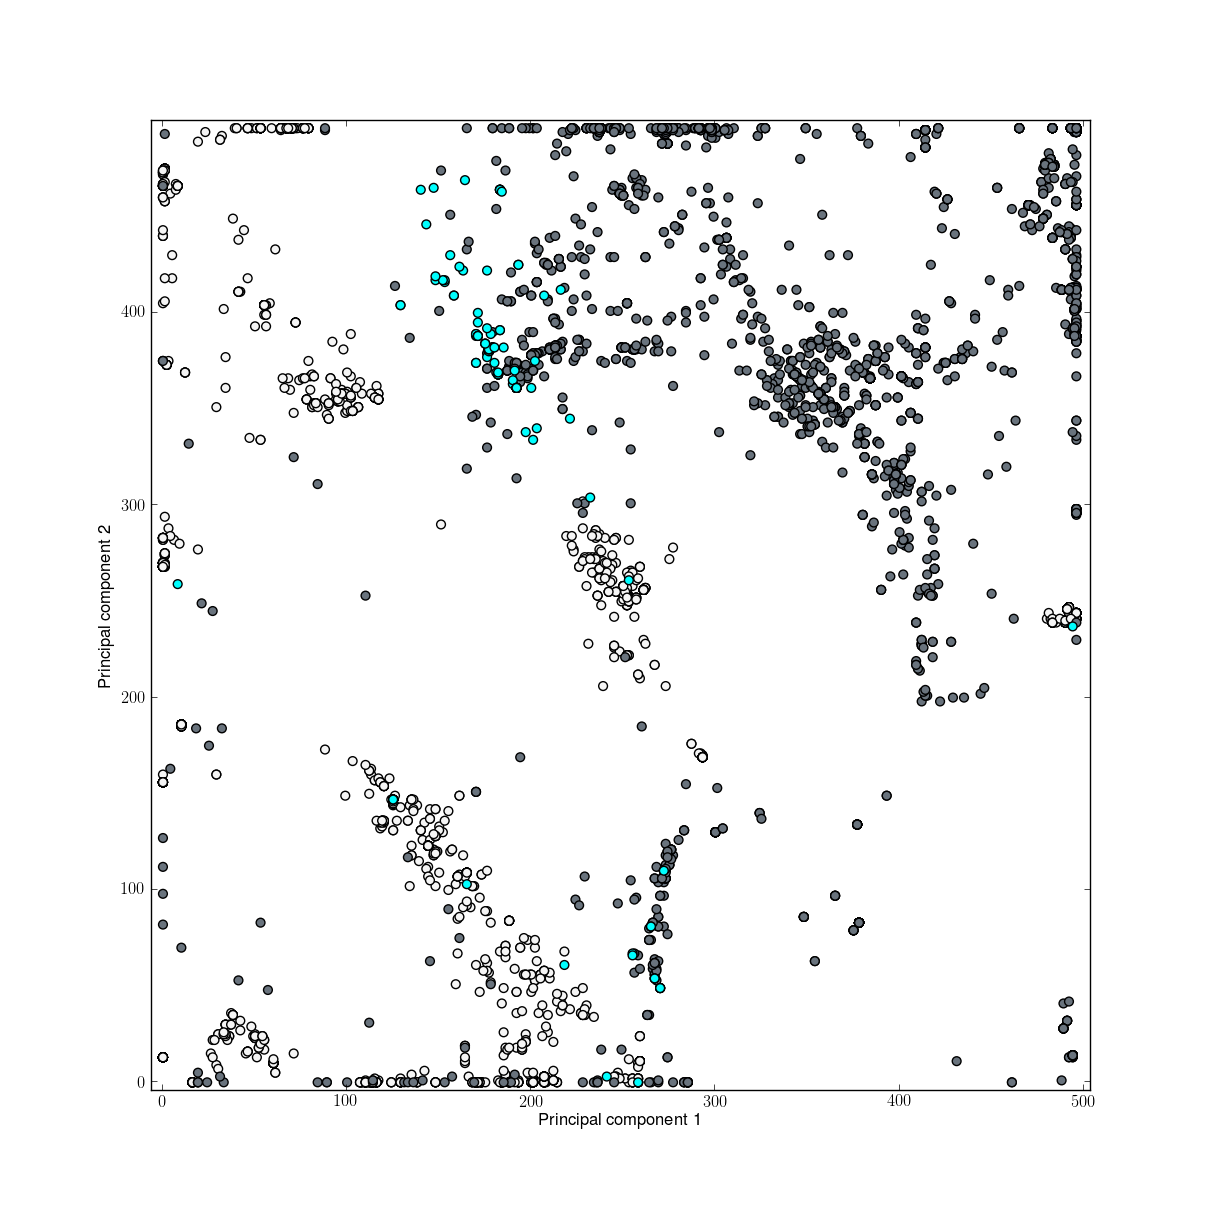
\includegraphics[trim=3cm 3cm 2cm 2cm,clip, width=\textwidth]{./img/SOM2.png}
	\subcaption{$SOM$}\label{figSOM}
	\end{minipage}
	\begin{minipage}{0.50\textwidth}
	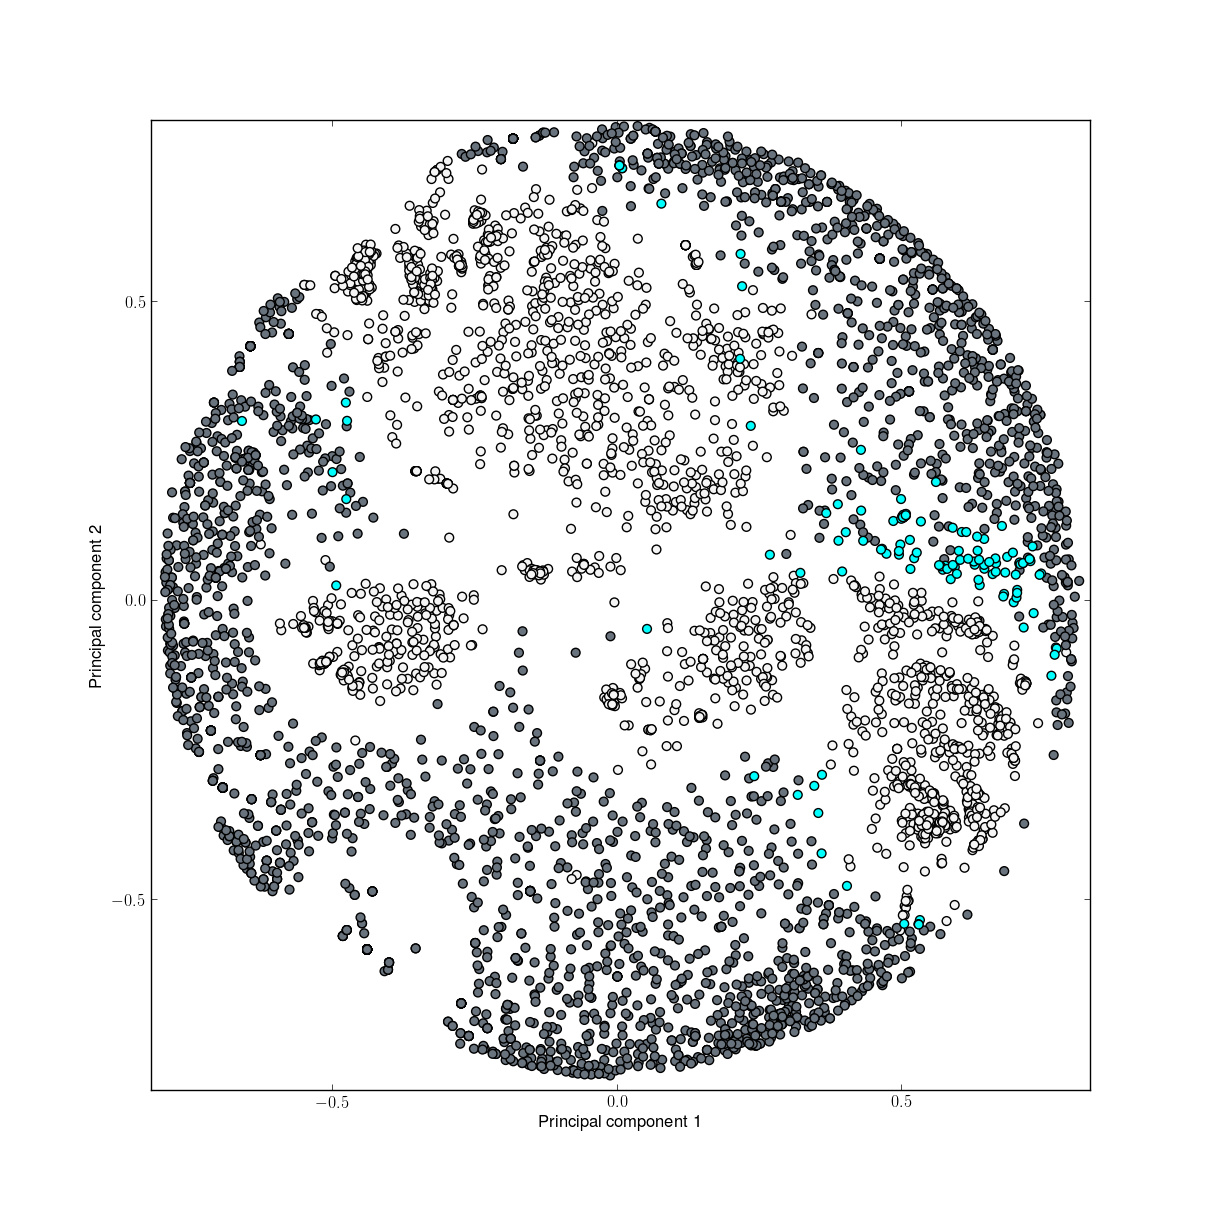
\includegraphics[trim=3cm 3cm 2cm 2cm, clip, width=\textwidth]{./img/MDS_cosine.png}
	\subcaption{$MDS$}\label{figMDS}
	\end{minipage}	

	\caption[Projection de l’ensemble des réplicons]{Projection de l’ensemble des réplicons $V^{R}$\\ \medskip Coloration selon le type de réplicon: chromosome (gris clair), plasmide (gris foncé), RECE (bleu).} 
\end{figure}  

Les algorithmes SOM et MDS produisent une organisation cohérente des réplicons bactériens (Table \ref{tabscorevisu}; Figures \ref{figSOM} et \ref{figMDS}). Ils fournissent une meilleure organisation taxonomique des chromosomes que les ACP et ISOMAP, et réussissent à structurer les réplicons plasmidiques (Table \ref{tabscorevisu}). La distance \textit{cosine}, utilisée par les deux méthodes SOM et MDS, ne tient compte que des attributs non-nuls des observations, et produit des distances pertinentes entre plasmides et chromosomes ainsi qu’entre plasmides. Cette structuration n'est de plus pas influencée par le biais d’échantillonnage des données car elle est également observée sur $\bar{V}^{R}_{genre}$ Figures \ref{figSOMnorm} et \ref{figMDSnorm}). 
 
\begin{figure}[H]
	\begin{minipage}{0.50\textwidth}
	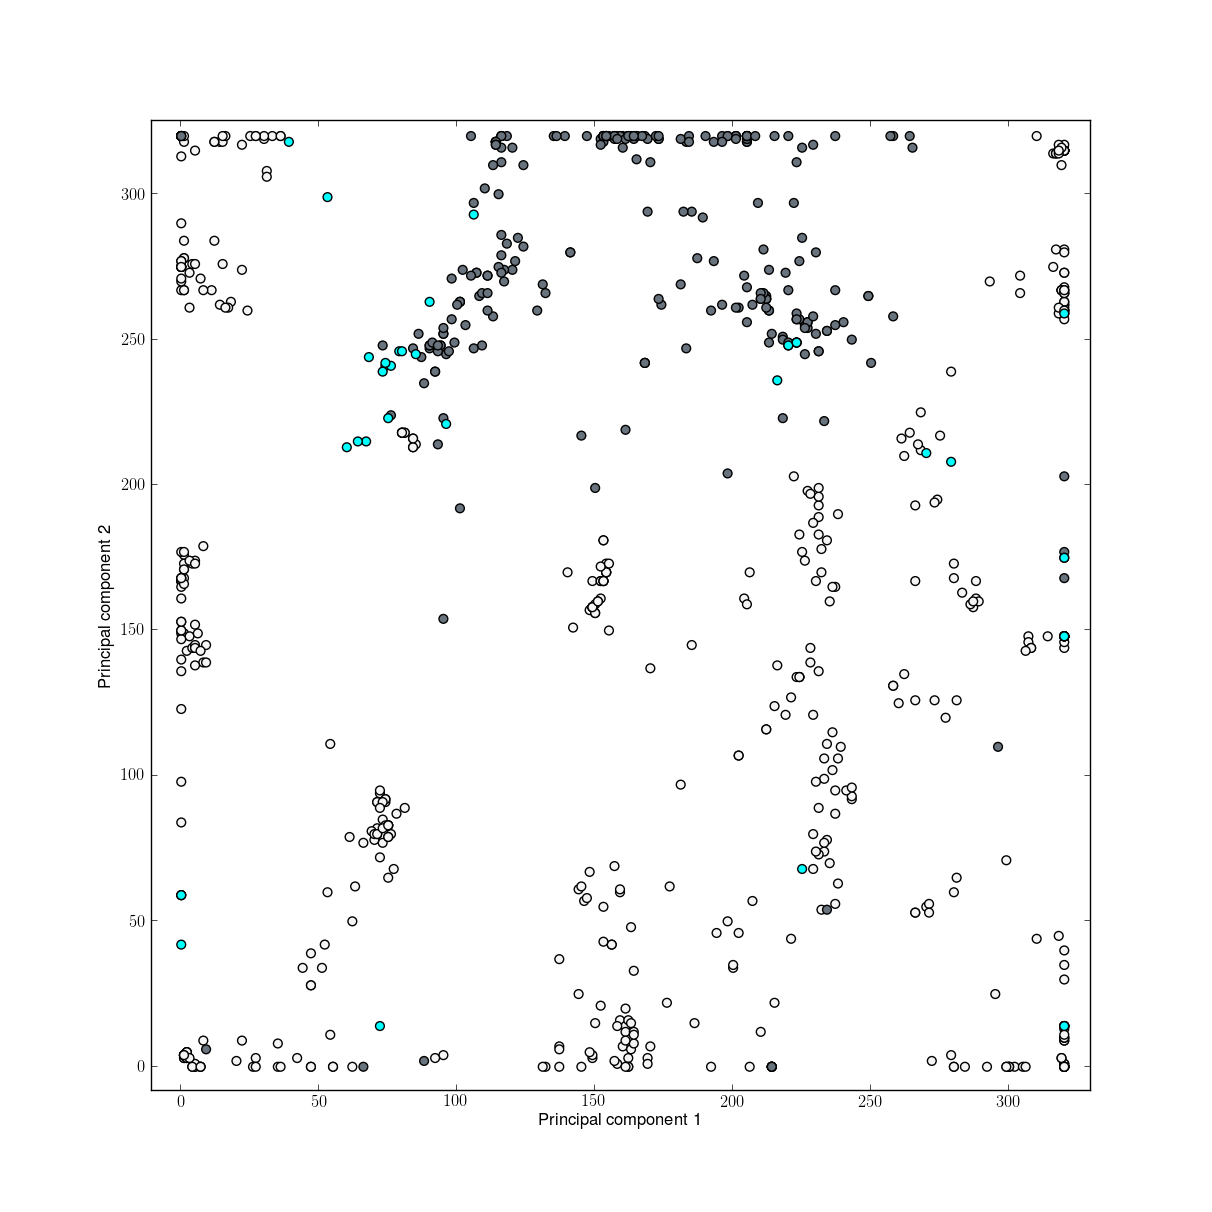
\includegraphics[trim=3cm 3cm 2cm 2cm,clip,width=\textwidth]{./img/SOM_norm.png}
	\subcaption{$SOM$ sur $\bar{V}^{R}_{genre}$}\label{figSOMnorm}
	\end{minipage}
	\begin{minipage}{0.50\textwidth}
	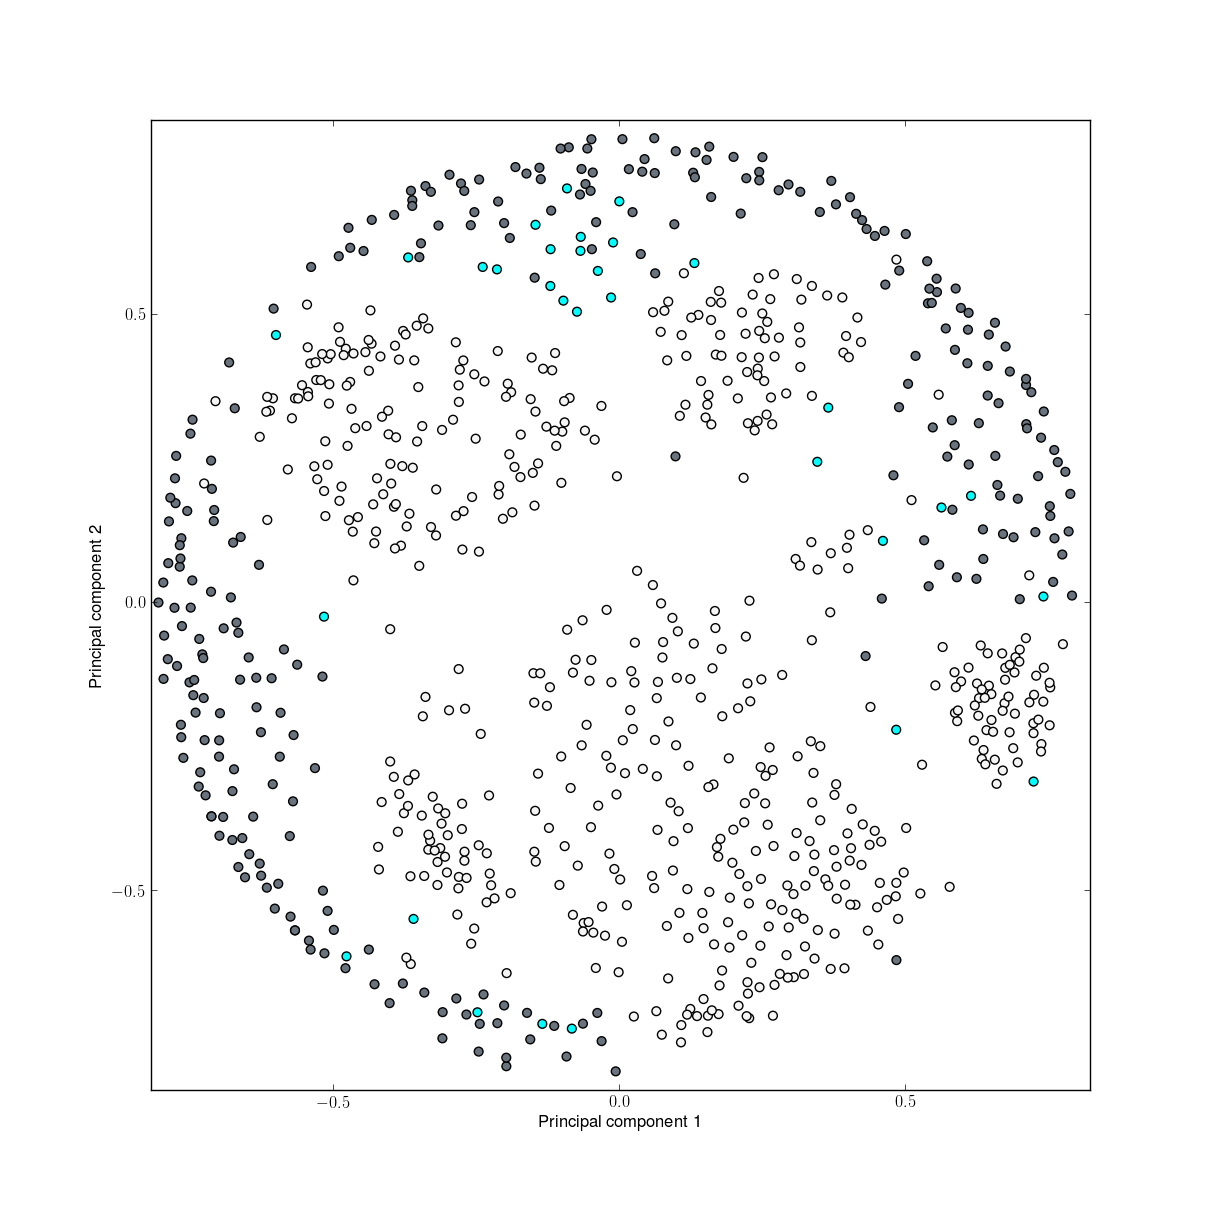
\includegraphics[trim=3cm 3cm 2cm 2cm,clip, width=\textwidth]{./img/MDS_cosine_norm.png}
	\subcaption{$MDS$ sur $\bar{V}^{R}_{genre}$}\label{figMDSnorm}
	\end{minipage}
	\caption[Projection des réplicons normés par genre bactérien]{Projection des réplicons normés par genre bactérien $\bar{V}^{R}_{genre}$\\\medskip Coloration selon le type de réplicon : chromosome (gris clair), plasmide (gris foncé), RECE (bleu).}
\end{figure}  

En prenant un ensemble de cellules $D$ assez large, la SOM parvient à discriminer les plasmides entre eux. Cependant un désavantage non négligeable de la SOM par rapport au MDS est le nombre d'itérations nécessaire (60.000), donc un temps de calcul conséquent, pour produire des résultats robustes.
\\
Concernant les RECE, on peut observer que:
\begin{description}
\item[$\blacktriangleright$] \textbf{\color{orange}Les RECE se placent généralement au niveau de l'interface entre chromosomes et plasmides} et semblent donc posséder des caractéristiques spécifiques les distinguant des plasmides (Figures \ref{figSOM}, \ref{figMDS}, \ref{figSOMnorm} et \ref{figMDSnorm}).
\item[$\blacktriangleright$] \textbf{\color{orange} Quelques RECE montrent une proximité singulière avec les chromosomes.}
\item[$\blacktriangleright$] Même si la séparation plasmide/chromosome est nette, il semble exister une proximité entre les plasmides et les chromosomes dont les hôtes appartiennent au même groupe taxonomique, par exemple, pour des groupes tel que les alpha-, bêta- ou gamma-protéobactéries (Figures \ref{figSOM2} et \ref{figMDS2}).

\begin{figure}[H]		
	\begin{minipage}{0.50\textwidth}		 	
	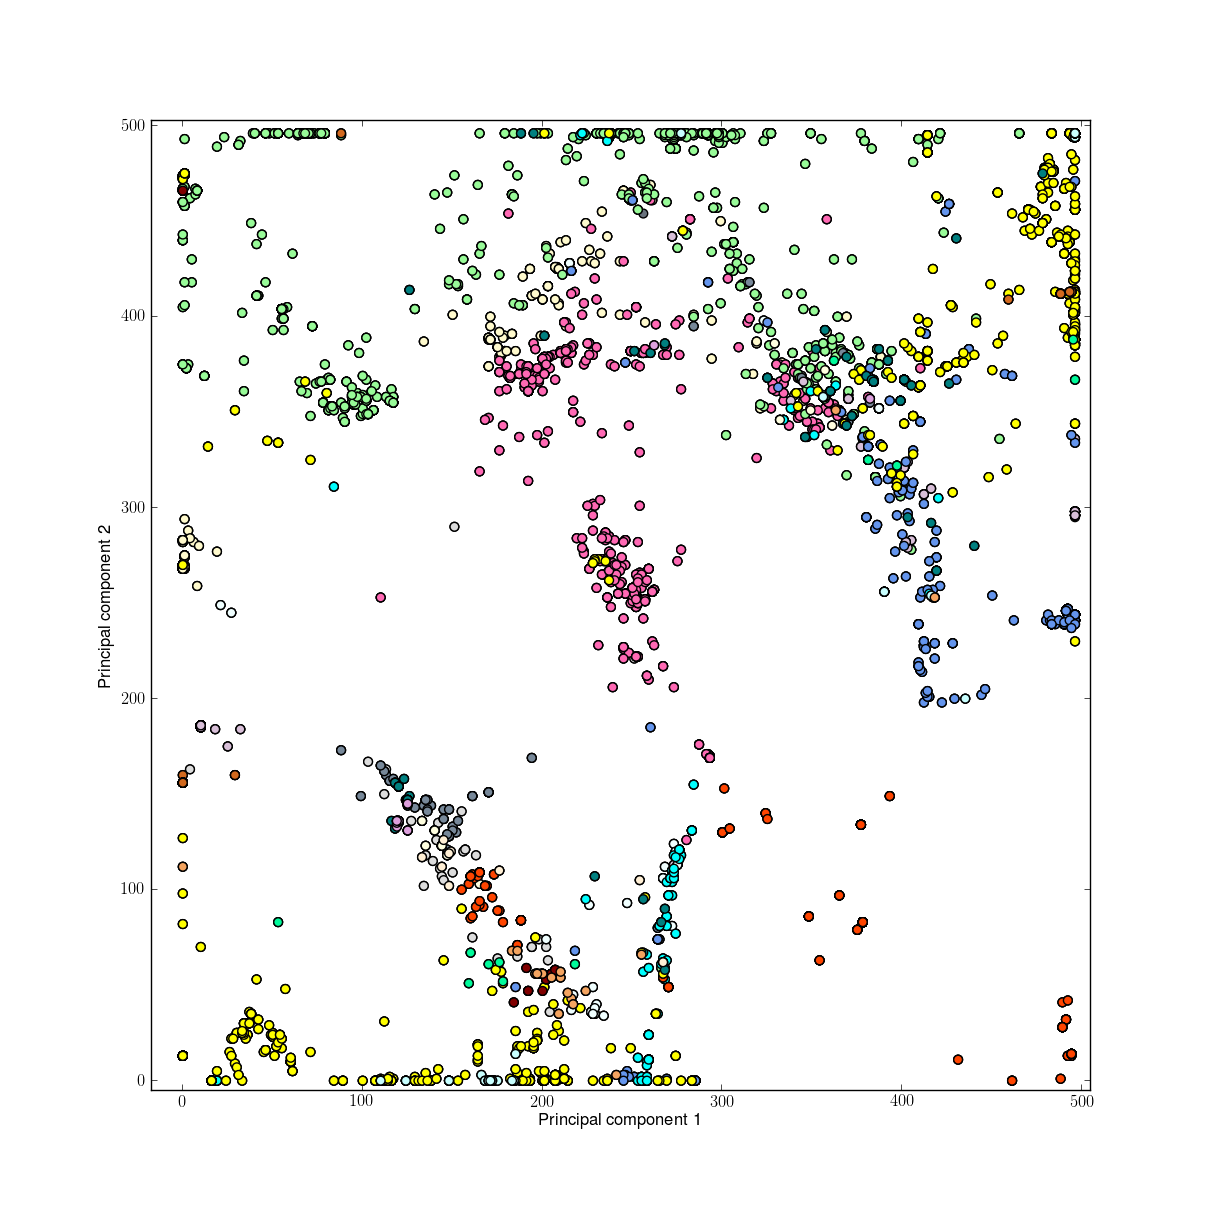
\includegraphics[trim=4cm 3cm 2cm 2cm,clip, width=\textwidth]{./img/SOM2_taxa.png}
	\subcaption{$SOM (2)$}\label{figSOM2}
	\end{minipage}
	\begin{minipage}{0.50\textwidth}
	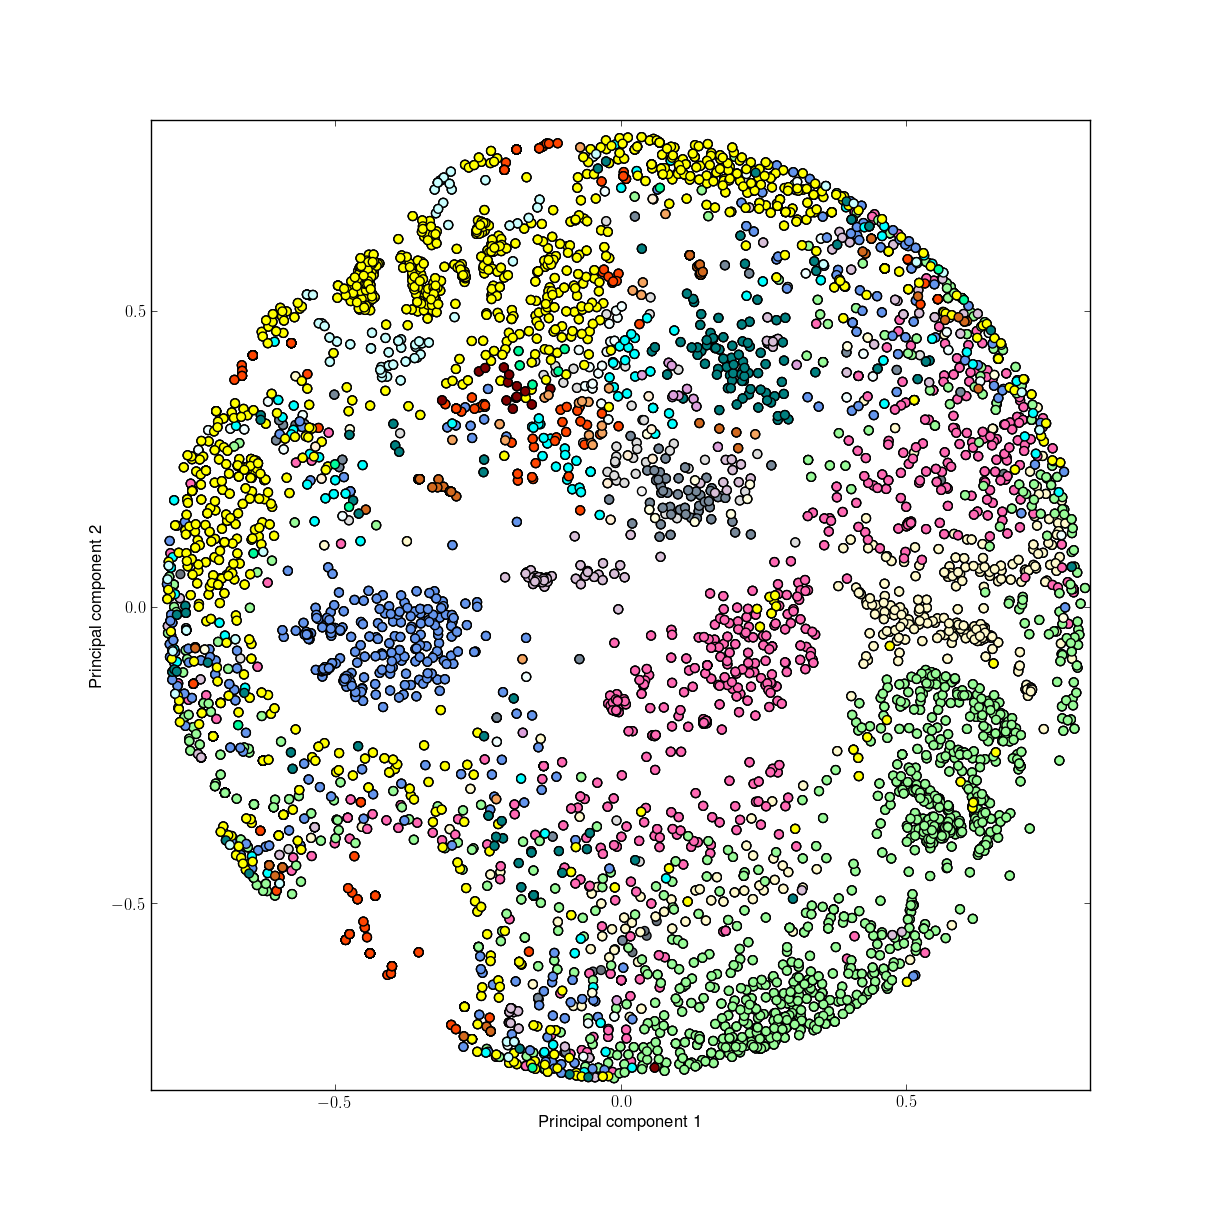
\includegraphics[trim=4cm 3cm 2cm 2cm,clip, width=\textwidth]{./img/MDS_taxa.png}
	\subcaption{$MDS (2)$}\label{figMDS2}
	\end{minipage}
	\caption[Identification des lignées bactériennes sur la projection des réplicons]{Représentation des lignées bactériennes sur les projections de l’ensemble des réplicons $V^{R}$ \\\medskip  Coloration selon la taxonomie de la bactérie-hôte : Acidobactéries (jaune transparent), Actinobactéries (bleu), Bacteroidetes (vert émeraude), Chlamydiae (orange foncé), Chlorobi (rose pâle), Chloroflexi (orange pâle), Cyanobactéries (cyan), Deinococcus-Thermus (bleu transparent), Firmicutes (jaune), Fusobactéries (vert), Planctomycètes (beige clair), Protéobacteries: Alpha (rose), Bêta (jaune pâle), Delta (gris foncé), Epsilon (violet pâle), et Gamma (vert clair), Spirochètes (rouge), Ténéricutes (bleu pâle), Thermotogae (marron foncé), Autres (gris pâle).}
\end{figure}  

\item[$\blacktriangleright$] \textbf{Cette proximité entre chromosomes et plasmides d'un même groupe taxonomique témoigne du flux intra-génomique de gènes liés aux STIG entre plasmides et chromosomes.}
\end{description}   

 \subsection{Graphes}
	En utilisant l'éq. \ref{eqbipartite}, $V^{R}$ et $\bar{V}_{genre}^{R}$ sont transformés en graphes bipartites, qui sont ensuite visualisés par des techniques dédiées de visualisation des graphes. Elles consistent à représenter les nœuds et arcs/arêtes des graphes par des points et flèches/traits entre les points dans un espace à deux ou trois dimensions. L’épaisseur des traits peut être une fonction de la pondération. Des algorithmes de topologie ou \textit{layout} organisent la  disposition des nœuds dans l'espace selon différentes stratégies. L’une d’entre elles est le \textit{force-directed layout} où un système de forces est appliqué à chaque nœud en fonction de ses arêtes. Le graphe est alors mis en mouvement jusqu'à ce qu'il atteigne un état stable. Ce  dernier dépend de la connectivité inter-nœud et peut être assimilé, par analogie, à l'action d'un champ de force (gravité, interaction électrostatique,...) sur une molécule, lui faisant adopter sa configuration la plus stable. L'algorithme que nous avons employé pour visualiser nos graphes est \textit{ForceAtlas2} \citep{jacomy2011forceatlas2}.
	%Dans un deuxième temps, $V^{R}$ et $\bar{V}_{genre}^{R}$ sont transformé en graphes bipartites en utilisant l'éq. \ref{eqbipartite}. Les graphes obtenus sont ensuite visualisées en utilisant les techniques de visualisation des graphes. Ces techniques consiste à représenter les nœuds et arcs/arêtes des graphes généralement par des points et flèches/traits entre les points dans un espace en 2 ou 3 dimensions, leur épaisseur pouvant être une fonction de leur pondération. La visualisation des graphes consiste à utiliser des algorithme de topologie ou \textit{layout}   organisant disposition des nœuds  dans l'espace selon différentes stratégies. Une de ces stratégies sont les \textit{force-directed layout} où un système de forces est appliqué à chaque noeud en fonctions de ses arêtes. Le graphe est alors mis en mouvement jusqu'à ce qu'il atteigne un état stable. Cet état stable dépend de la \textit{connectivité} inter-noeud et peut être assimilé, par analogie, à l'action d'un champ de force (gravité, interaction électrostatique,...) sur une molécule lui faisant adopter la configuration dans laquelle celle-ci est la plus stable. L'algorithme utilisée dans la visualisation des graphes est \textit{ForceAtlas2} \citep{jacomy2011forceatlas2}.  
		
\subsubsection{Graphes: résultats}\label{graphres}
	L'analyse des graphes formés pour $V^{R}$ (Figure \ref{figgrapherepl}) et des sous-graphes des différents groupes taxonomiques contenant des espèces multipartites (Figure \ref{figgprahe2}) apporte un autre point de vue que les projections en permettant d'analyser plus précisément les différentes interconnections de chaque réplicon par rapport aux clusters de protéines. L'utilisation du logiciel de visualisation Gephi, par ses nombreuses fonctionnalités, a apporté une contribution non négligeable dans la fouille de données des graphes.\\

 La quasi-majorité des réplicons sont interconnectés, témoignant de l'hérédité partagée des gènes des STIG présents dans les génomes bactériens. Plasmides et chromosomes semblent cependant clairement appartenir à des communautés différentes. Il existe néanmoins pour certains phyla une interconnection forte entre chromosomes et plasmides. Est passé en revue ci-dessous les observations tirées de l'analyse des graphes pour les génomes multipartites. À cause de la grande complexité des données, seulement les observations les plus marquantes visuellement sont rapportées. 
 
 \begin{description}
 \item[Protéobactéries] Différents niveaux de connections des RECE avec les plasmides et chromosomes existent chez les protéobactéries (détaillés ci-dessous). Les RECE des Protéobactéries sont interconnectés \textit{via} certains clusters remarquables, notamment les clusters annotés IciA, Lrp, FtsE, AcrA ou HN-S (Figure \ref{figconnectiv}). De manière générale, les RECE fortement interconnectés avec les plasmides le sont \textit{via} les clusters annotés ParA/ParB, Rep et en lien avec les systèmes PSK.

 	\begin{itemize}
 	\item[\textbf{Alpha}] Les RECE sont liés pour part à de nombeux clusters plasmidiques dont ceux annotés ParA, ParB et RepC, témoignant de la proximité avec les plasmides de type RepABC présents chez les Alphaprotéobactéries. Cependant, ilsi sont liés à des clusters typiquement chromosomiques, FtsK (pour les RECE de \textit{Brucella} et d'\textit{Agrobacterium}) et ParE (pour les RECE de \textit{Brucella}) notamment. Il existe des clusters spécifiques des RECE, annotés TyrK, FtsE ou AcrA particulièrement. Enfin, l'interconnection des RECE de \textit{Paracoccus} et de \textit{Asticcacaulis} avec des réplicons chromosomiques est surprenante (Figure \ref{figalpha}). Les RECE des \textit{Brucella} forment un groupe distinct alors que ceux de \textit{Sphingobium} semblent plus interconnectés avec des plasmides.
 	% Les gènes des STI suggérés comme étant transférés entre le chromosome et les plasmides ancestrales des Rhizobiales \citep{Slater2009} sont retrouvés sur les RECE correspondant. 
 	\item[\textbf{Bêta}] Les RECE se distinguent clairement des chromosomes et des plasmides en formant un groupe homogène distinct (Figure \ref{figbeta}). Ils partagent différents clusters avec les plasmides tels que ceux annotés parA ou Xer, entre autres. Les RECE sont interconnectés aux chromosomes \textit{via} de nombreux clusters tels que FtsI, IciA ou Rob. Il existe des différences entre les RECE I et les RECE II des \textit{Burkholderia}, ces derniers semblant plus interconnectés aux plasmides.Il est à noter que les RECE I des \textit{Burkholderia} sont liés à des clusters annotés DnaG connectés aux chromosomes (sauf ceux des \textit{Burkholderia}), témoignant d'un probable transfert ancestral du chromosome vers le RECE I. 
 	\item[\textbf{Gamma}] Les RECE sont connectés à l'interface des chromosomes et plasmides (Figure \ref{figgamma}). Ceux de \textit{Pseudoalteromonas} sont moins interconnectés avec les RECE des \textit{Vibrio/Aliivibrio} et \textit{Photobacterium} soulignant leur origine distincte.
 	\end{itemize}
\item[Acidobactéries] Le RECE de \textit{Candidatus} Chloroacidobacterium thermophilum est interconnecté aux chromosomes par ParA/ParB, DnaB, AcrA, ScpB principalement, et n'est pas interconnecté avec les plasmides des Acidobactéries. Il est cependant connecté à des plasmides d'autres phylum \textit{via} des clusters Rep, Helicase ou PSK principalement.
 \item[Actinobactéries] Le RECE de \textit{Nocardiopsis dassonvillei} est interconnecté aux chromosomes \textit{via} de nombreux clusters annotés principalement FtsE, FtsK, FtsW, FtsI, MinD et ParA.
 \item[Bacteroidetes] Les RECE de \textit{Prevotella} sont interconnectés aux chromosomes \textit{via} de très nombreux clusters et ont peu d'interconnections avec les plasmides.
 \item[Chloroflexi] Les RECE de \textit{Sphaerobacter thermophilus} et \textit{Thermobaculum terrenum} sont interconnectés aux chromosomes et aux plasmides \textit{via} de nombreux clusters. En particulier, le RECE de \textit{S. thermophilus} est lié aux clusters DnaA (GI: 269929006), DnaG et FtsI. 
 \item[Cyanobactéries] Deux configurations distinctes sont trouvées chez les RECE de \textit{Anabaena} et \textit{Cyanothece}: le RECE de \textit{Anabaena} est assez interconnecté aux chromosomes \textit{via} des clusters annotés FstI, DnaG, FtsE, CpbA, MreB, ParA entre autre. Inversement le RECE de\textit{Cyaothece} interconnecté aux plasmides \textit{via} des clusters de type Xer, ParA et helicase notamment.
\item[Deinococcus-Thermus] Le RECE de \textit{Deinococcus} est lié à huit clusters annotés ParA, ParB, FtsE, Helicase, XerC et HupB. Par le nombre de clusters et par son interconnection, Il est beaucoup plus proche des autres plasmides de \textit{Deinococcus}. Il est cependant interconnecté aux chromosomes \textit{via} les clusters FtsE et HupB notamment et est lié à un nombre (trois) relativement élevé de cluster FtsE. 
 \item[Firmicutes] Le RECE de \textit{Butyrivibrio proteoclasticus} est connecté aux plasmides \textit{via} des clusters annotés Rep et PSK principalement et est connecté aux chromosomes \textit{via} ceux annotés DnaB, Rob, FtsE, Xer. pCY186, un plasmide de \textit{B. proteoclasticus} est attaché au même cluster DnaB, ainsi qu'à deux clusters annotés DnaA (GI: 302668636 et 302668625).
 \item[Spirochètes] Les RECE de \textit{Leptospira} sont liés chacun à trois ou qutre clusters de protéines pour un total de six clusters différents. Les clusters en commun sont annotés ParA et ParB et ceux n'étant pas présents sur tous les RECE sont annotés XerD et HupB. Le cluster annoté ParA est lié exclusivement aux chromosomes des spirochètes, avec une exception: un plasmide de \textit{Turneriella}. Aucun des six clusters n'est lié à un autre plasmide des Spirochètes. Les RECE possèdent de plus deux gènes appartenant à ce cluster. 
\end{description}  
 
\begin{landscape}
\thispagestyle{plain}
\begin{figure}
\vspace{-2cm}
\hspace{-2cm}
\begin{minipage}[t]{0.5\linewidth}
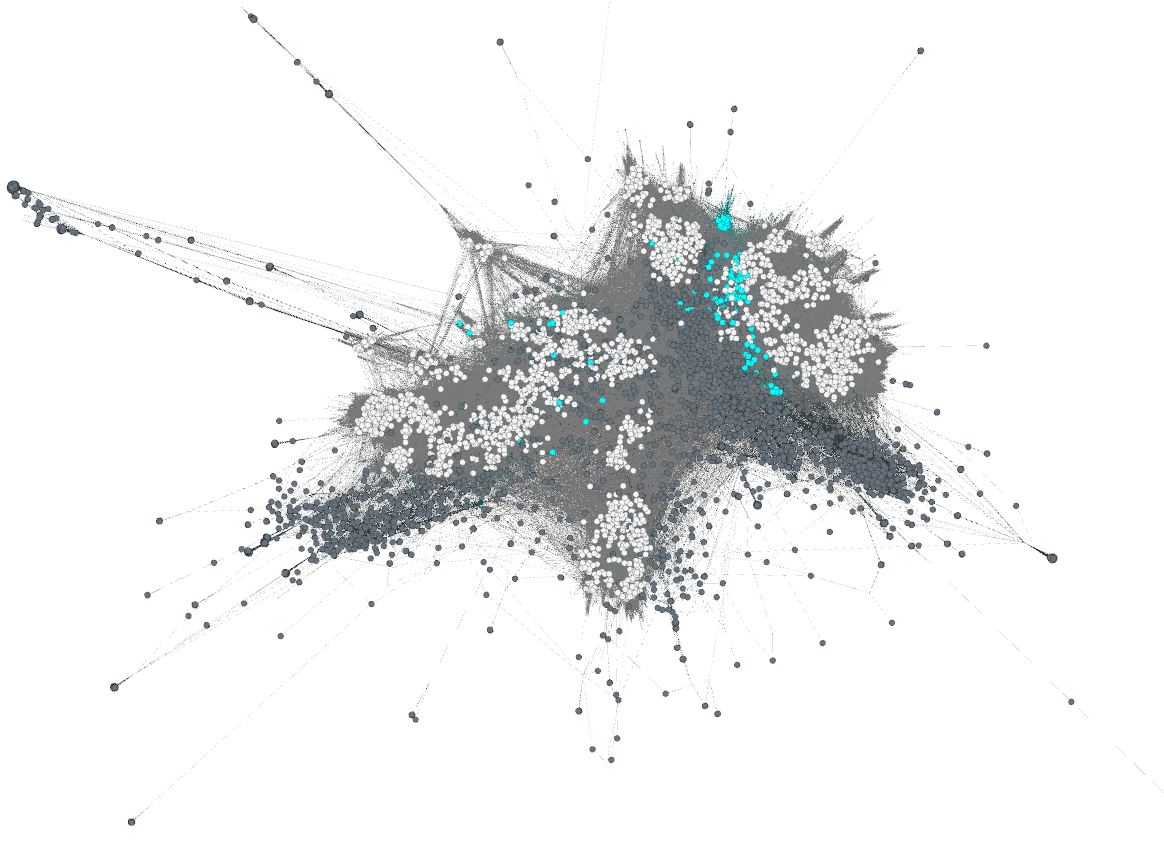
\includegraphics[width=1.13\textwidth ]{./img/graph_all_grey_white_cyan.png}
\subcaption{Type de réplicons}\label{figrepltype}
\end{minipage}
\hspace{1.5cm}
\begin{minipage}[t]{0.5\linewidth}
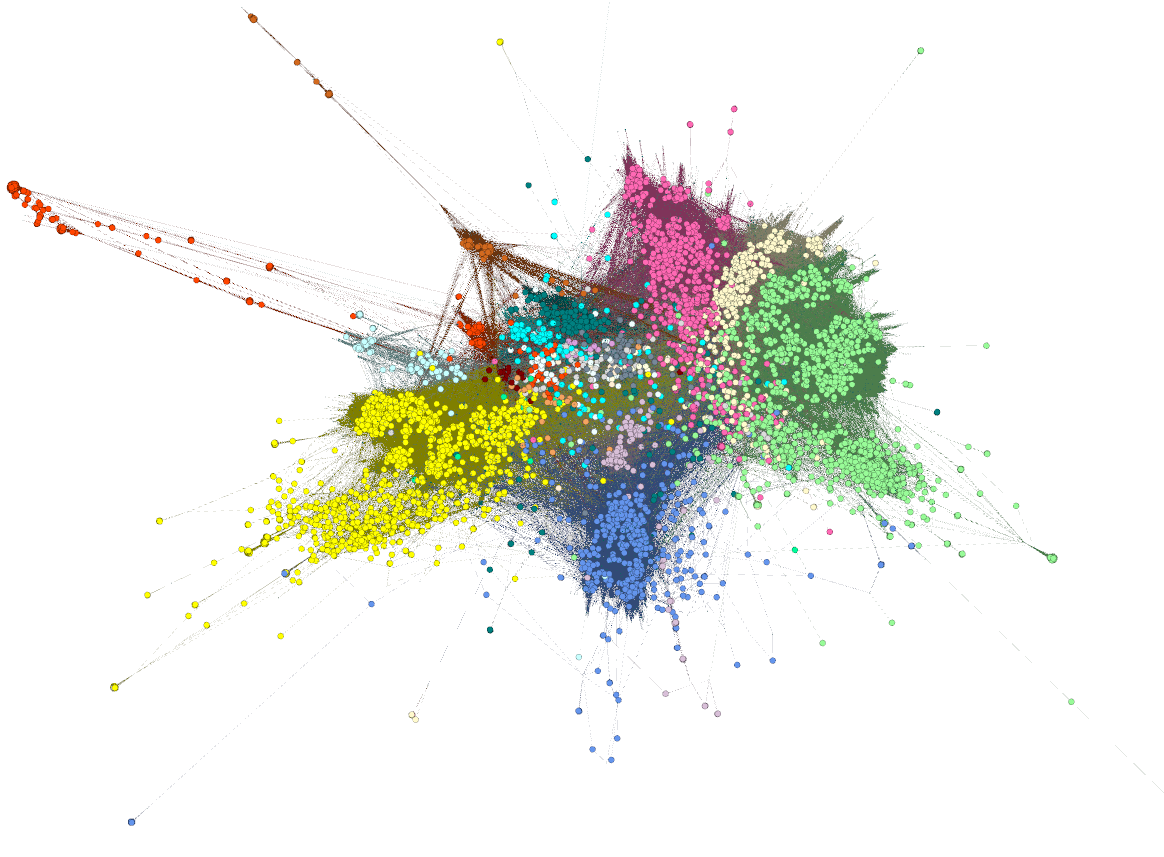
\includegraphics[width=1.13\textwidth ]{./img/graph_all_taxa_color_whitefont.png}
\subcaption{Phylum/Classe des bactéries-hôtes}\label{figreplphyl}
\end{minipage}
\caption[Visualisation des réplicons par graphe bipartite]{Visualisation des réplicons par graphes bipartites.\\\medskip \ref{figrepltype}. Selon le type de réplicon : chromosome (gris clair), plasmide (gris foncé), RECE (bleu). \ref{figreplphyl}. Selon la taxonomie de la bactérie-hôte : Acidobactéries (jaune transparent), Actinobactéries (bleu), Bacteroidetes (vert émeraude), Chlamydiae (orange foncé), Chlorobi (rose pâle), Chloroflexi (orange pâle), Cyanobactéries (cyan), Deinococcus-Thermus (bleu transparent), Firmicutes (jaune), Fusobactéries (vert), Planctomycètes (beige clair), Protéobacteries: Alpha (rose), Bêta (jaune pâle), Delta (gris foncé), Epsilon (violet pâle), et Gamma (vert clair), Spirochètes (rouge), Ténéricutes (bleu pâle), Thermotogae (marron foncé), Autres (gris pâle).}\label{figgrapherepl}
\end{figure}
\end{landscape}


\begin{landscape}
\thispagestyle{empty}
\begin{figure}
\vspace{-3cm}
\begin{center}
\begin{minipage}[t]{0.40\textwidth}
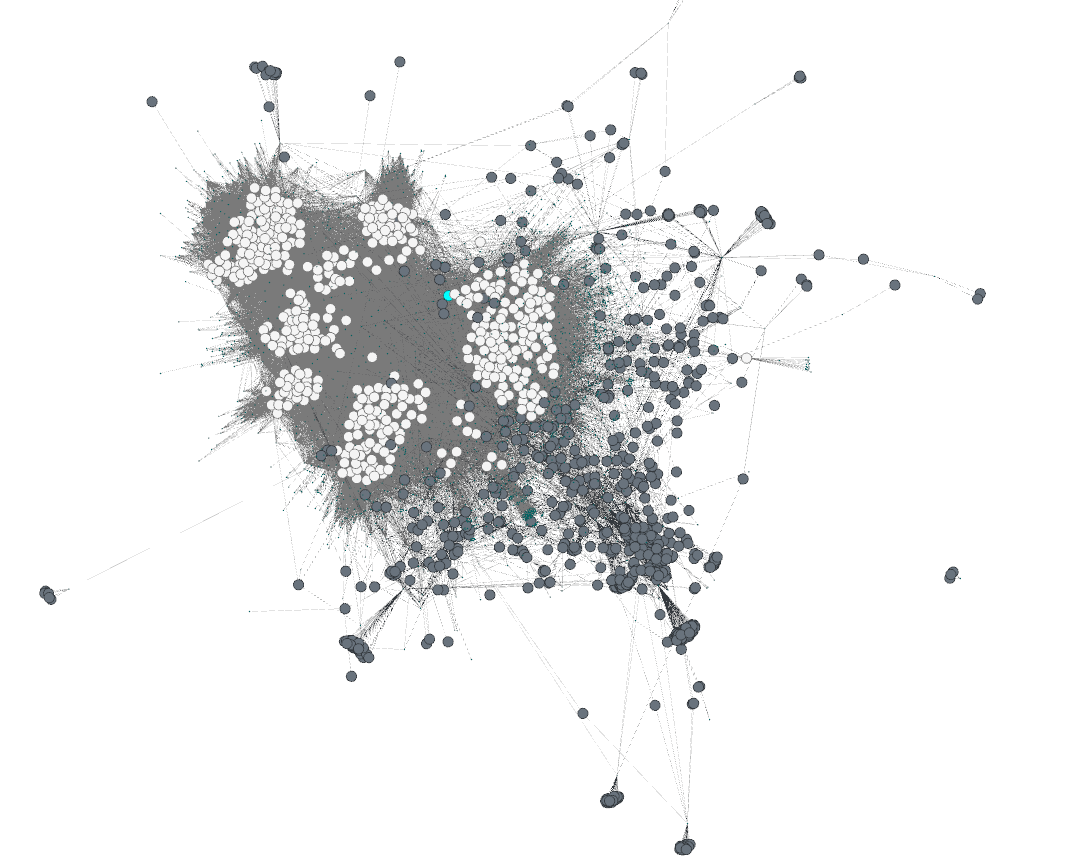
\includegraphics[width=\textwidth]{./img/clostrid.png}
\subcaption{Firmicutes}\label{figclost}
\end{minipage}
\begin{minipage}[t]{0.40\textwidth}
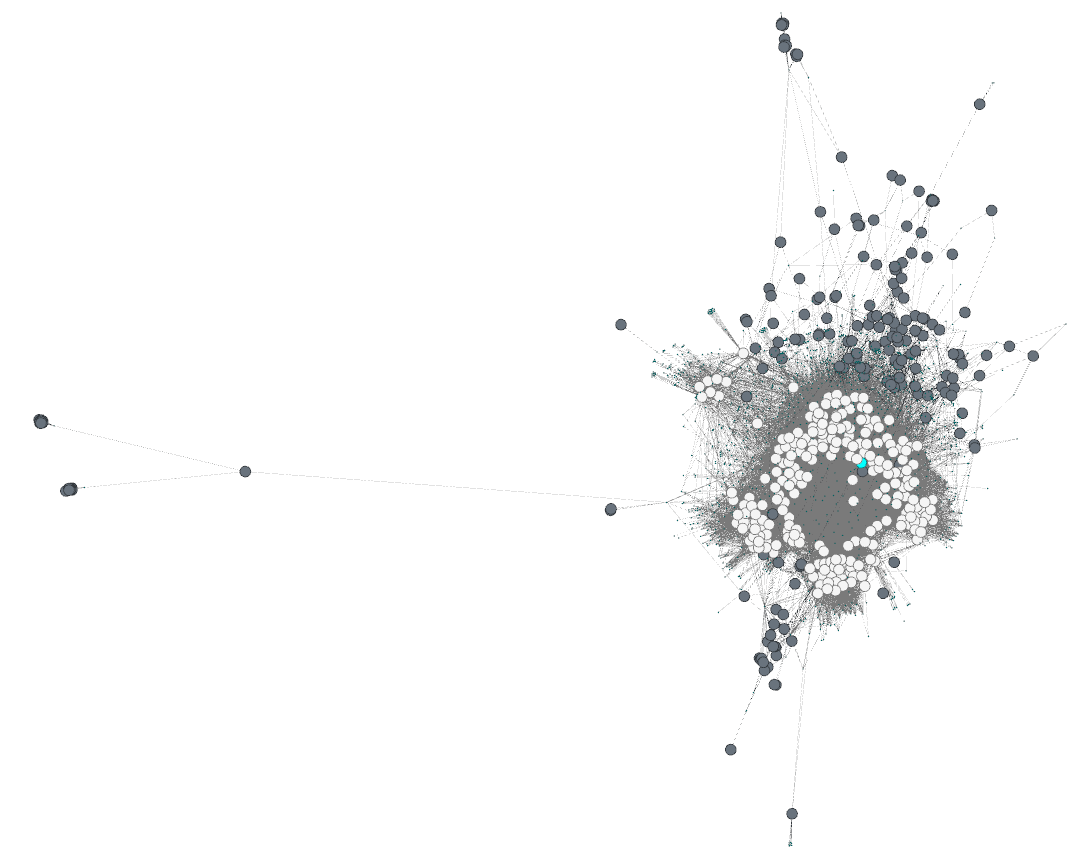
\includegraphics[width=\textwidth]{./img/actinobacter.png}
\subcaption{Actinobactéries}\label{figactino}
\end{minipage}
\begin{minipage}[t]{0.40\textwidth}
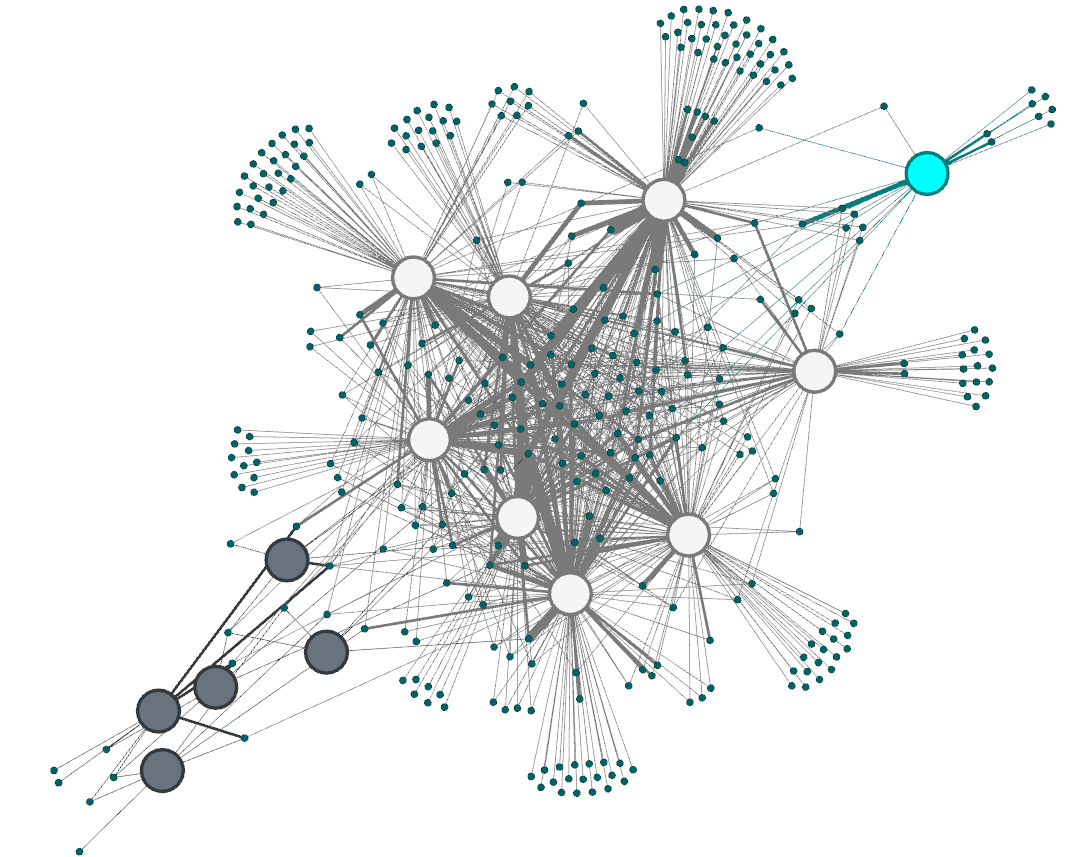
\includegraphics[width=\textwidth]{./img/acido.png}
\subcaption{Acidobactéries}\label{figacido}
\end{minipage}
\begin{minipage}[t]{0.40\textwidth}
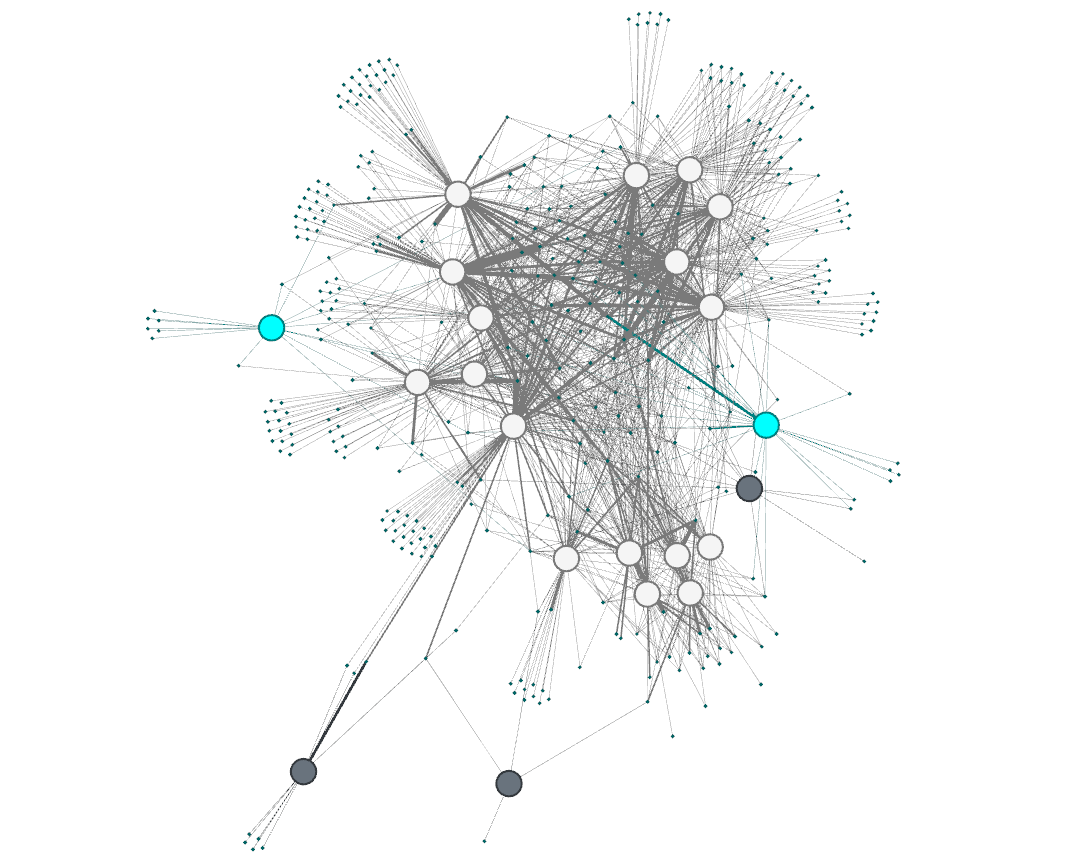
\includegraphics[width=\textwidth]{./img/chloroflex.png}
\subcaption{Chloroflexi}\label{chloro}
\end{minipage}
\\
\vspace{0.2cm}
\begin{minipage}[t]{0.40\textwidth}
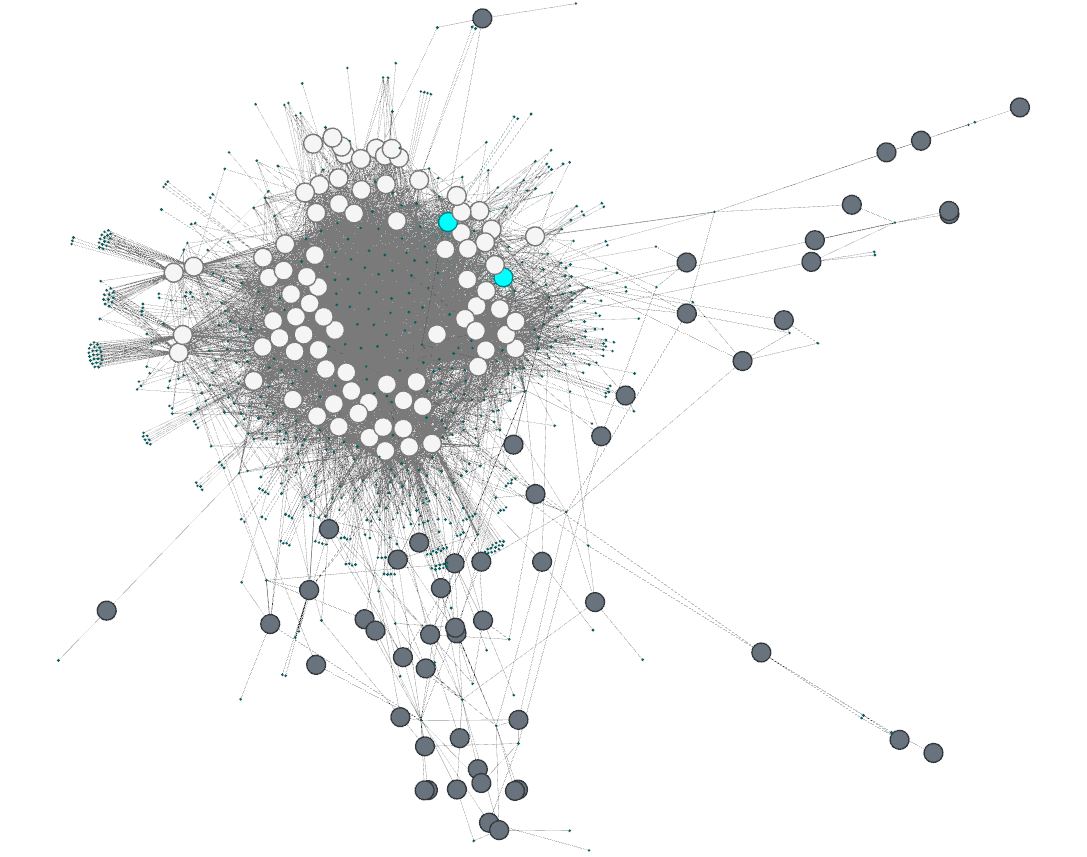
\includegraphics[width=\textwidth]{./img/BCF.png}
\subcaption{Bacteroidetes}\label{figbact}
\end{minipage}
\begin{minipage}[t]{0.40\textwidth}
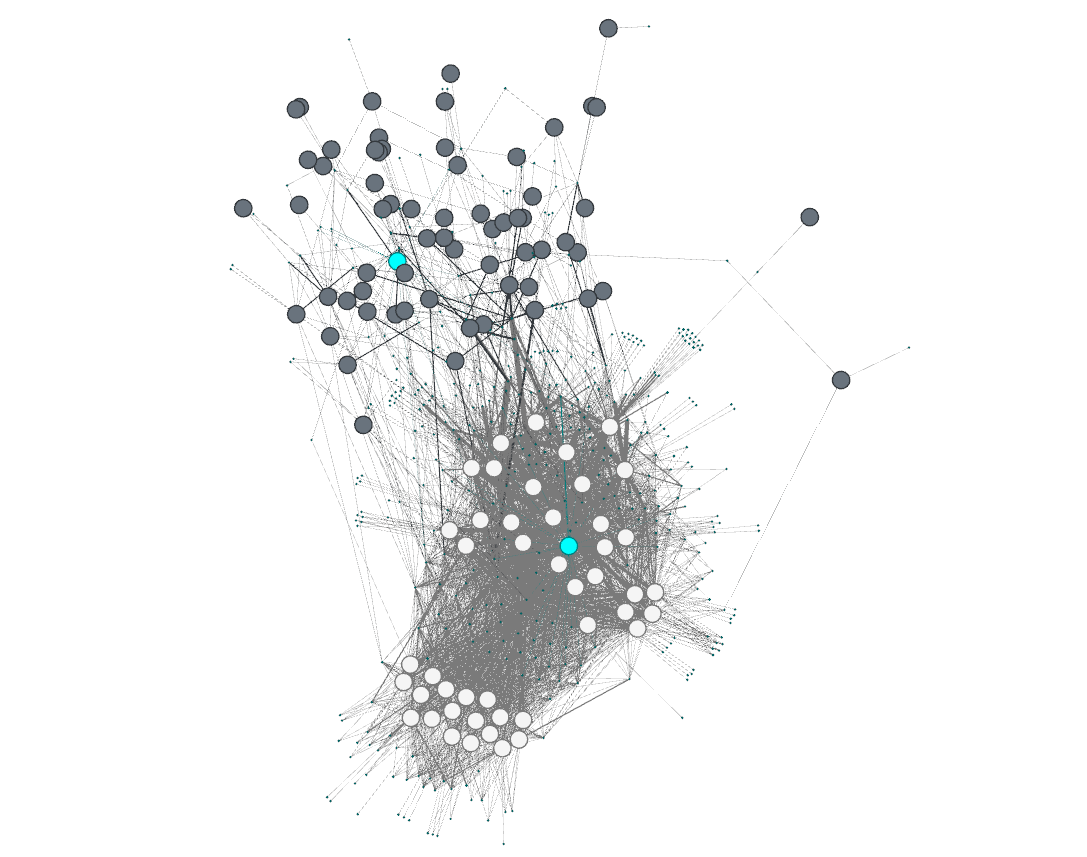
\includegraphics[width=\textwidth]{./img/cyano.png}
\subcaption{Cyanobactéries}\label{figcyano}
\end{minipage}
\begin{minipage}[t]{0.40\textwidth}
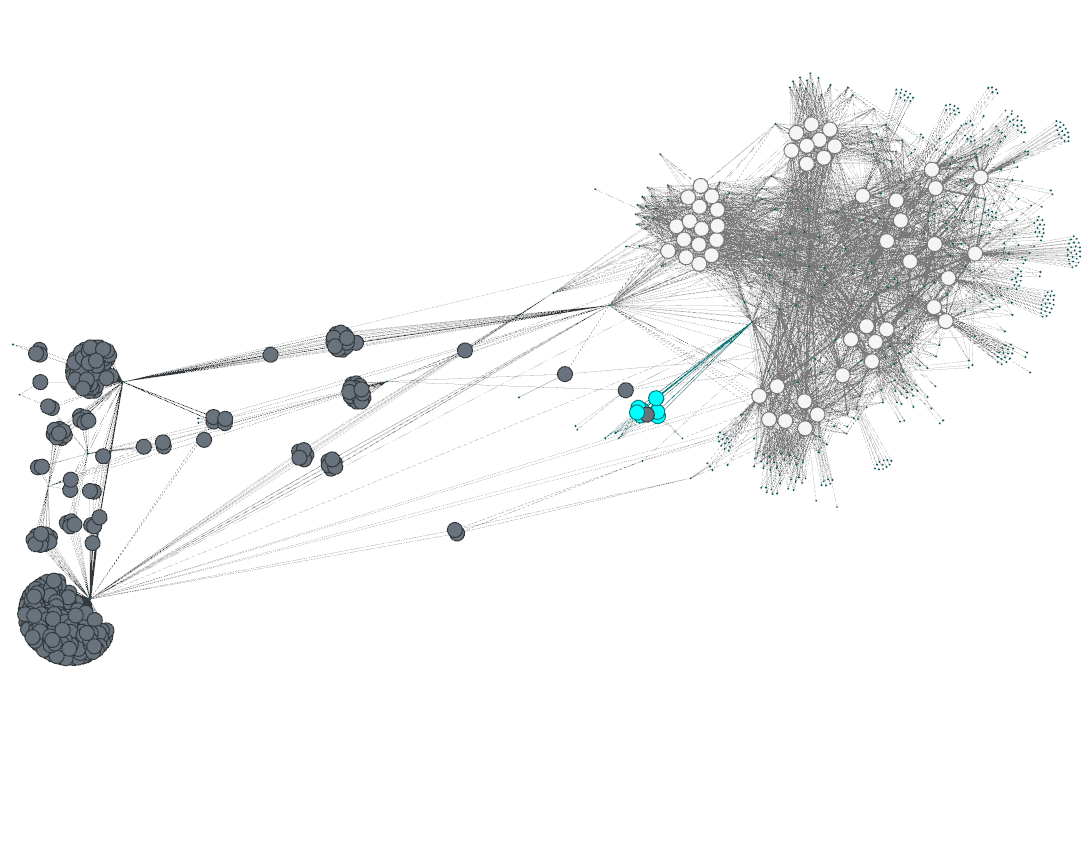
\includegraphics[width=\textwidth]{./img/leptospir.png}
\subcaption{Spirochètes}\label{figspiro}
\end{minipage}
\begin{minipage}[t]{0.40\textwidth}
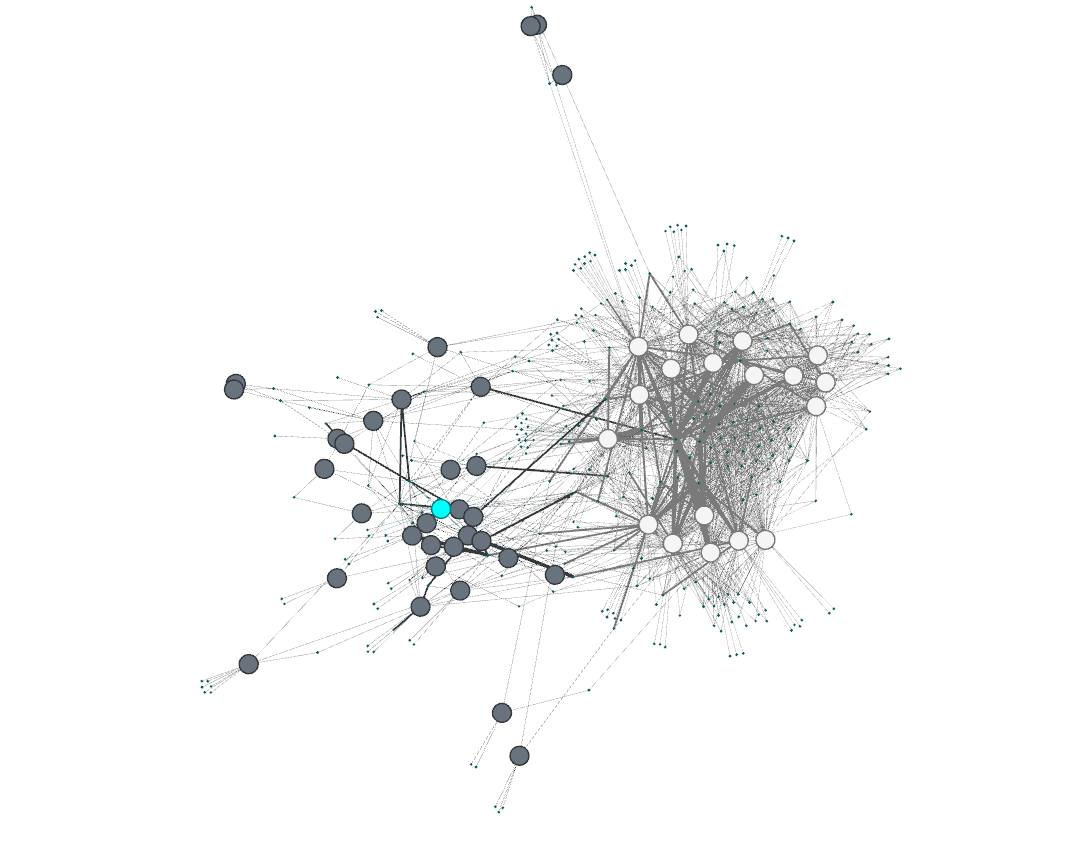
\includegraphics[width=\textwidth]{./img/deinococcus.png}
\subcaption{Deinococcus-Thermus}\label{figdeino}
\end{minipage}
\\
\vspace{0.2cm}
\begin{minipage}[t]{0.40\textwidth}
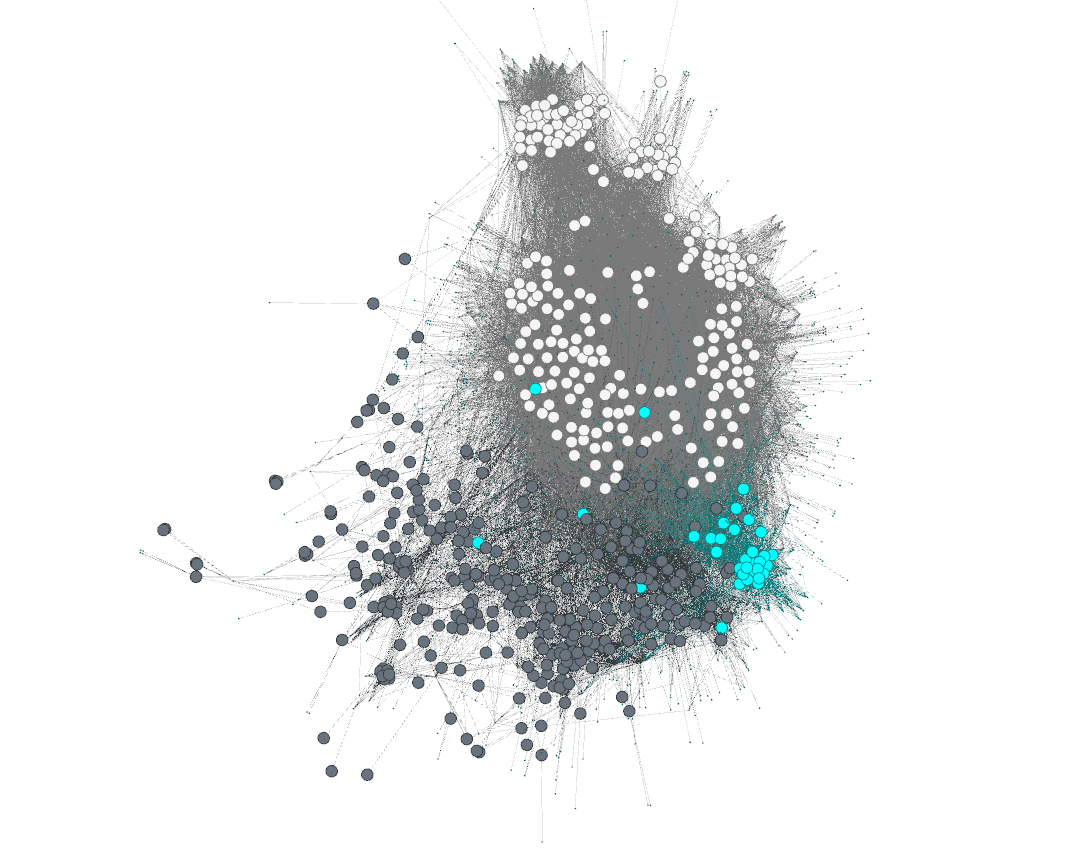
\includegraphics[width=\textwidth]{./img/alpha.png}
\subcaption{Alphaprotéobactéries}\label{figalpha}
\end{minipage}
\begin{minipage}[t]{0.40\textwidth}
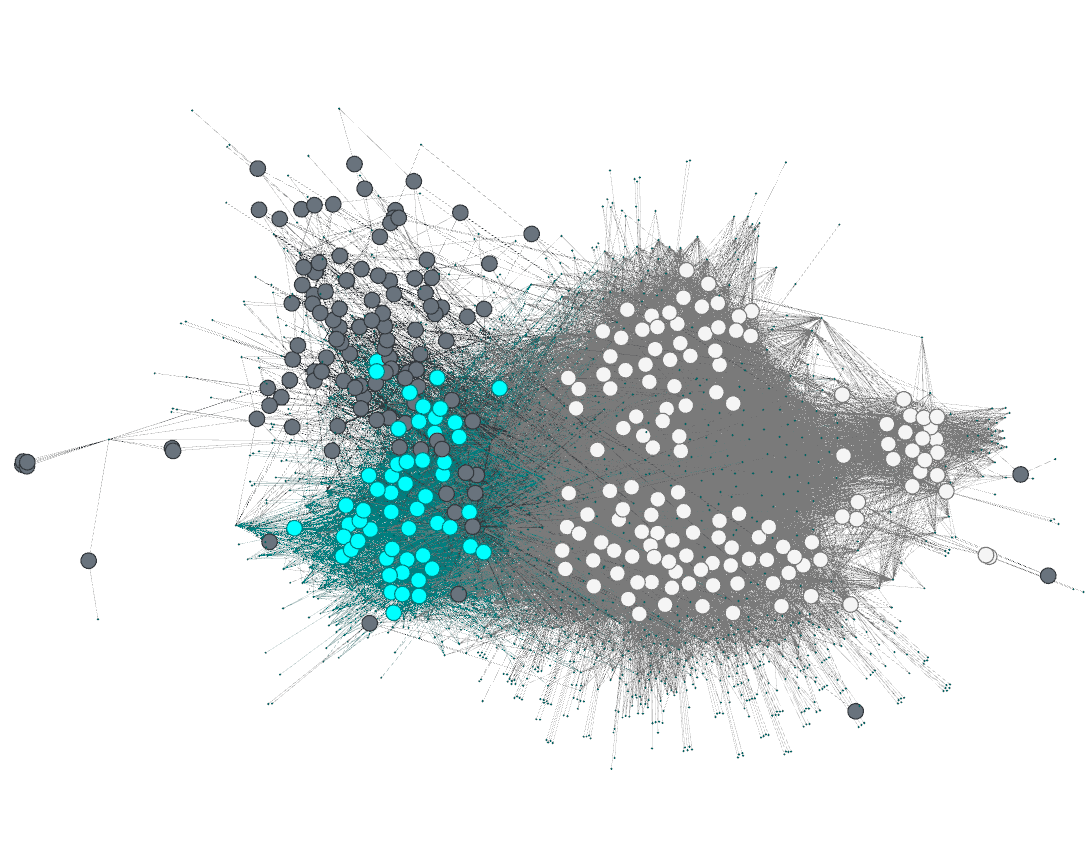
\includegraphics[width=\textwidth]{./img/beta.png}
\subcaption{Bêtaprotéobactéries}\label{figbeta}
\end{minipage}
\begin{minipage}[t]{0.40\textwidth}
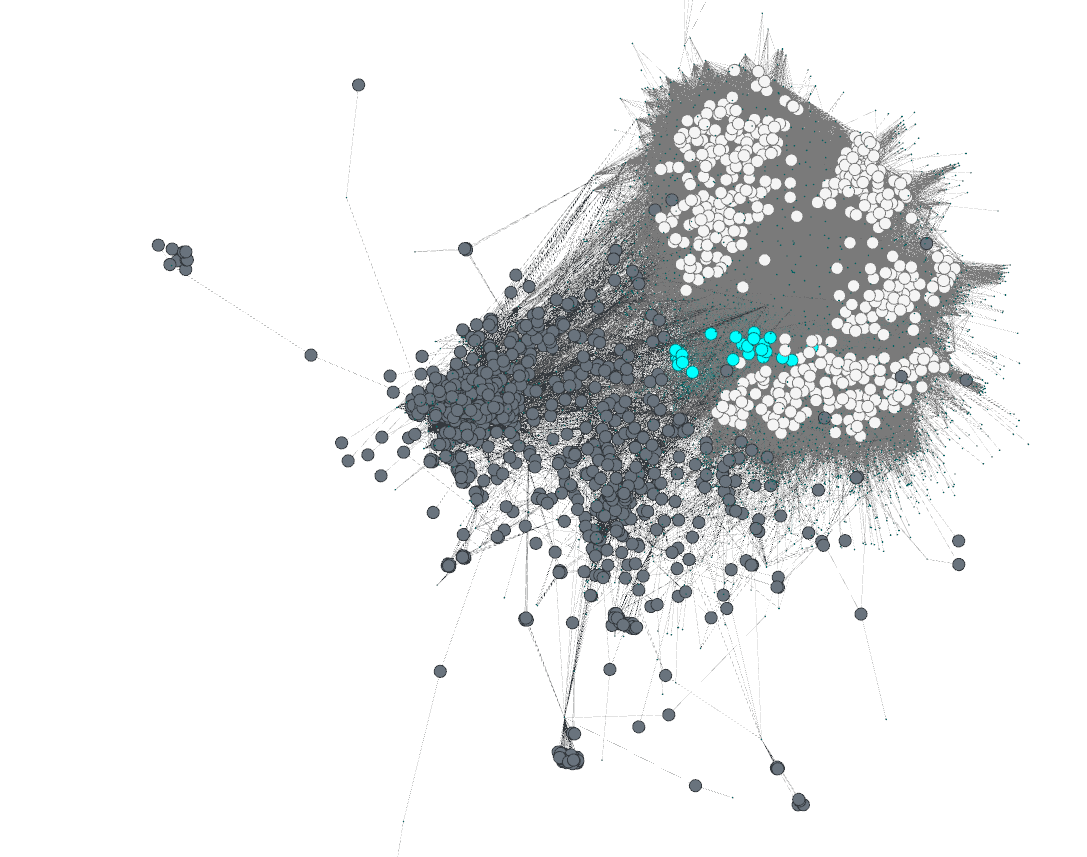
\includegraphics[width=\textwidth]{./img/gamma.png}
\subcaption{Gammaprotéobactéries}\label{figgamma}
\end{minipage}
\caption[Visualisation par graphe des réplicons par lignée bactérienne]{Visualisation par graphe bipartite des réplicons $V^{R_{taxon}}$ selon la taxonomie de leur hôte (phylum ou classe pour les Protéobactéries).\\\medskip Coloration selon le type de réplicon : chromosome (gris clair), plasmide (gris foncé), RECE (bleu). Les clusters de protéines (vert foncé) sont visibles pour certaines résolutions.} \label{figgprahe2}
\end{center}
\end{figure}
\end{landscape}


\begin{figure}[H]
\hspace{-2cm}
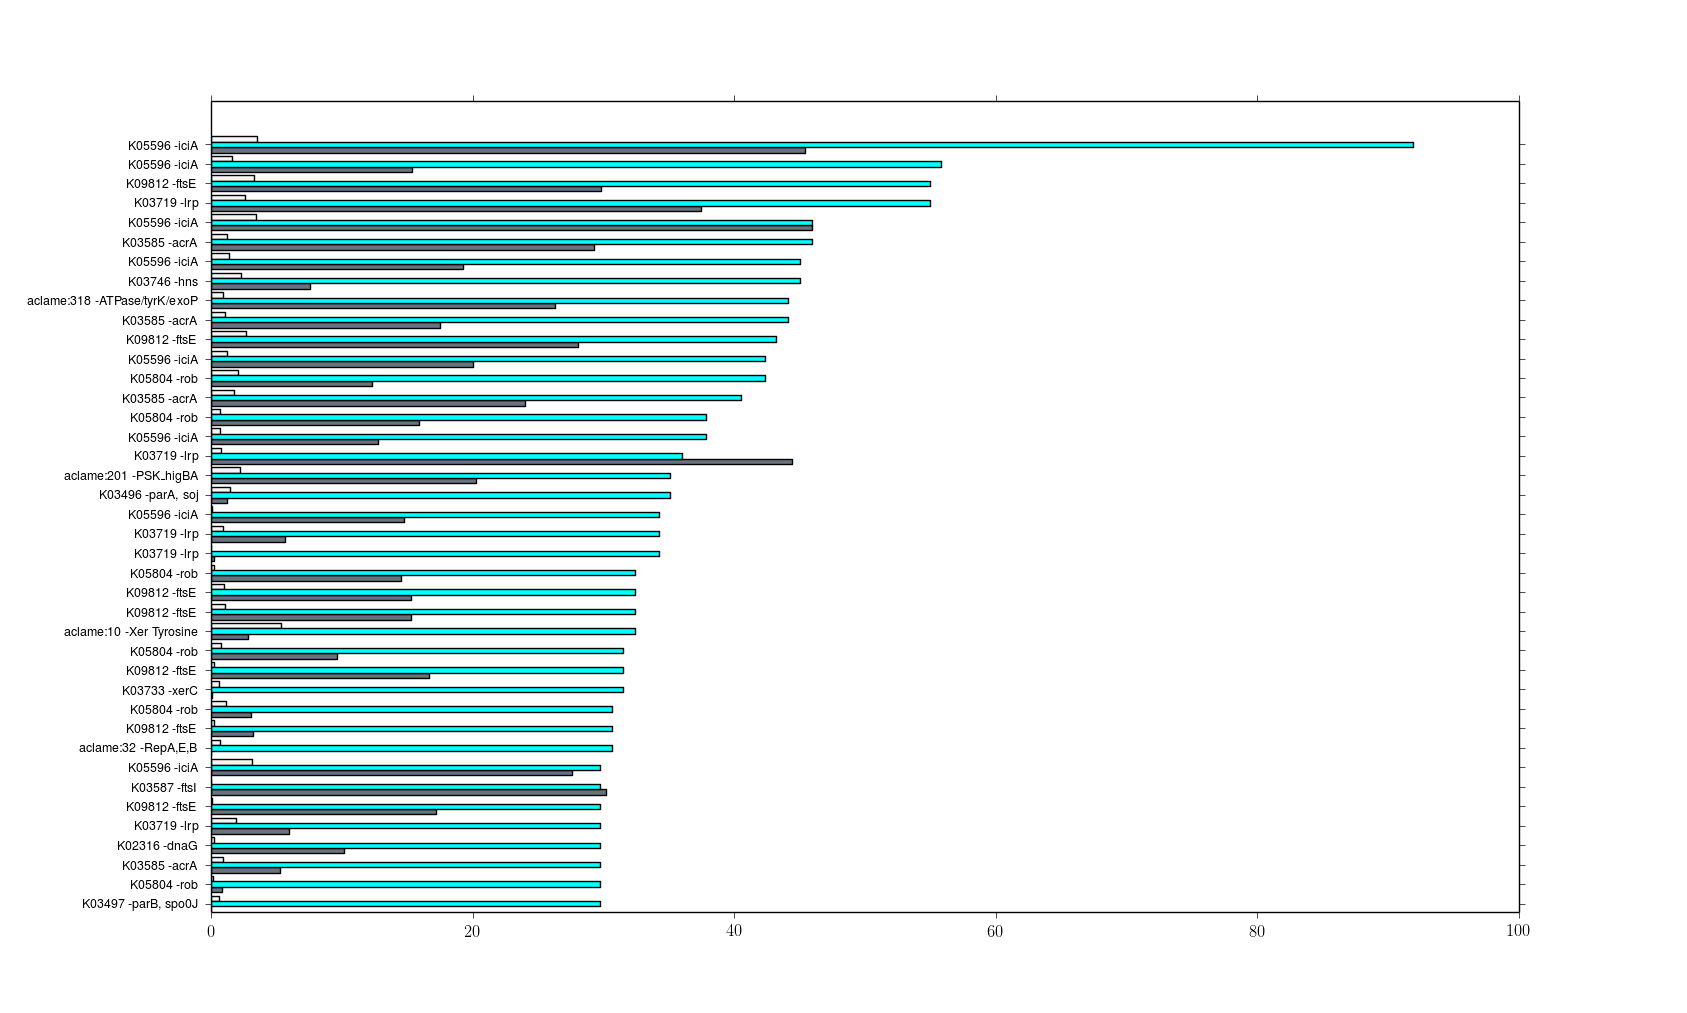
\includegraphics[trim=0cm 1cm 0cm 0cm,clip,width=1.2\textwidth, height=0.7\textheight]{./img/cluster_connectivity2.png}
%\mbox{\footnotesize\hspace{4cm} Pourcentages d'observations connectées aux clusters (par type)}
\caption[Pourcentages de connexion aux clusters de protéines par type de réplicon]{Pourcentages, par type de réplicon, de connexion aux 40 clusters de protéines les plus connectés aux observations annotées en tant que RECE de $\bar{V}^{R_{\textrm{Protéobactéries}}}_{genre}$. Pour chaque cluster (ordonnée), sont représentés les pourcentages de connexion (abcisse) pour les observations annotées en tant que RECE (bleu), chromosome (gris foncé) et plasmide (gris clair).}\label{figconnectiv}
\end{figure} 

   Dans l'interprétation visuelle des graphes obtenus par ForceAtlas2, un des biais vient du positionnement de certains plasmides faiblement connectés dans certains groupes de chromosomes hautement connectés s'ils sont liés à des clusters de protéines communs. Il est de plus difficile de comparer la pertinence visuelle des graphes bipartites spatialisés avec les visualisations obtenues par projection. 

\subsubsection{Logiciels utilisés}
 \begin{description}
 \item[Gephi] \citep{Bastian2009} logiciel ``open source" de graphes, a été utilisé pour spatialiser (en utilisant ForceAtlas 2) et visualiser les graphes.
 \item[Python] a été utilisé pour réaliser les nombreux workflows, préparer les données, préparer les fichiers \textit{graphml} utilisés par Gephi. 
 \end{description}
 
 
 
\subsection{Visualisation: discussion}

  La projection des réplicons selon leurs STIG par MDS et SOM et la visualisation par graphe montrent que \textbf{\color{orange}les réplicons s'organisent par groupe taxonomique et selon leur type}. Même si les chromosomes et plasmides forment des groupes et communautés distinctes, ils partagent tout de même de nombreux gènes des STIG, témoignant de phénomènes d'échange génétique inter-réplicons dans les génomes bactériens. Les RECE semblent de plus posséder une distribution des gènes des STIG les distinguant des chromosomes et plasmides, et se positionnent à l'interface entre chromosomes et plasmides. Il existe différents degrés d'interconnection des RECE avec les chromosomes et les plasmides selon les RECE. \textbf{Cependant, compte tenu de la grande complexité des données, ces premiers résultats ne permettent pas d'identifier avec certitude des caractéristiques spécifiques des RECE. }
  
  
  
\section{Classification non-supervisée}\label{parclassifnonsupervis}
      L'analyse de clustering des réplicons bactériens a pour objectif principal d'étudier le comportement des RECE par rapport aux autres réplicons. Le positionnement de manière stable d'un RECE dans un groupe de chromosomes ou un groupe de plasmides indiquerait une proximité avec les membres de ce groupe. À l'inverse un cluster homogène de RECE peut être le témoin de leur spécificité et les différencier en tant qu'espèce moléculaire distincte des autres réplicons. 
      
 \subsection{Algorithmes de clustering}\label{paralgoclust}
      
      Différents algorithmes de clustering ont été testés, les critères retenus étant le temps d'exécution, l'implémentation ou l'implémentabilité, les performances mesurées et la stabilité. Pour prendre en compte la très haute dimensionalité des données, différentes approches ont été suivies:
      
      \begin{description}
       \item[i)] Algorithmes de clustering spécifiques pour des données en grandes dimensions 
       \item[ii)] Réduction de dimension initiale par projection des données puis clustering dans ce nouvel espace
	  \item[iii)] Clustering des graphes bipartites de $V^{R}$ et $\bar{V}^{R}_{genre}$.
       \end{description}

        Les méthodes de réduction de dimensions testées sont les mêmes que précédemment (Table \ref{tabprojec}) avec $q$, le nombre de dimensions, variable. Soient $Cl$ un clustering de $C$ clusters, $V$ un ensemble d'observations et $d$ une distance. La Table \ref{tabalgoclust} introduit brièvement les principaux algorithmes de clustering utilisés
.

\begin{longtable}{ @{\hspace{-2cm}} >{\bfseries}p{0.15\textwidth}@{\hspace{1cm}}|>{\small}p{\textwidth}}
      \caption[Algorithmes de clustering utilisés]{Principaux algorithmes de clustering utilisés dans l'analyse des données.}\\ \label{tabalgoclust}
      K-Means & \citep{hartigan1975clustering,hartigan1979algorithm} Algorithme de clustering des plus populaires. Le principe original consiste à minimiser l'erreur $E=\sum_{C \in Cl}\sum_{r \in C} d(v_{r},\bar{v}^{C})$. Les paramètres de l'algorithme étant la distance $d$, le nombre de clusters $k$, le nombre d'itérations et d'exécutions de l'algorithme et son mode de convergence. De nombreuses variantes de l'algorithme existent \citep{gan2007data}.
	\\[0.4cm]
     Classifieurs \mbox{Hiérarchiques} \mbox{Agglomératifs} (CHA)
      & Algorithmes partant d'un état initial où chaque observation est considérée comme une feuille (ou nœud terminal) d'un arbre, puis formant des clusters d'observations en fusionnant de façon itérative les feuilles de cet arbre \citep{gan2007data}. Différents critères peuvent être utilisés pour choisir la fusion optimale entre deux nœuds, comme par exemple la distance minimale, maximale ou moyenne entre les observations de deux nœuds, la distance entre les centroïdes des nœuds, ou la méthode WARD (\textit{cf.} ci-dessous). 
	\\[0.4cm]
     WARD & \citep{ward1963hierarchical,ward1963application} Algorithme de la famille des classifieurs hiérarchiques agglomératifs. À partir d'un ensemble de clusters intermédiaires, le principe de cette famille d'algorithmes est de fusionner deux clusters si et seulement si un certain critère objectif est minimal \citep{gan2007data}. La méthode de Ward consiste à regrouper deux clusters intermédiaires d'un clustering $Cl_{i}$ de façon à ce que l'inertie intra-cluster $I=\frac{1}{|Cl_{i}|}\sum_{C \in Cl}\sum_{r \in C}d^{2}(v_{r},\bar{v}^{C}) $ soit minimisée.
	\\[0.4cm]
     DBSCAN & \citep{ester1996density} Algorithme de clustering par densité. D'une manière itérative, une observation $r$ est ajoutée à un cluster existant $C$ si ceux-ci sont joignables par densité selon $d$, c'est-à-dire s'il existe une observation $r_{i} \in C$ telle que $d(v_{r},v_{r_{i}})\leqslant v_{seuil}$. Les paramètres de l'algorithme étant $d$, $v_{seuil}$ et le nombre de points minimum d'un cluster. Cet algorithme s'applique cependant difficilement aux données de dimensionalité élevée car elles sont alors éparpillées dans l'espace de représentation \citep{gan2007data} (voir aussi \ref{parfleau}).
	\\[0.4cm]
     SUBCLU & \citep{Vista2004} Algorithme de clustering des données de dimensionalité élevée. Le principe est d'exécuter une procédure DBSCAN dans les différents sous-espaces où les données sont joignables par densité. Les différents sous-espaces sont sélectionnés de façon similaire à l'algorithme \textit{a priori} \citep{agrawal1994fast}. Les paramètres de SUBCLU sont les mêmes que ceux de DBSCAN.
	\\[0.4cm]
     INFOMAP & \citep{rosvall2008maps} Algorithme de détection de communautés d'un graphe $G$. Les données étant transformées en graphe bipartite par la relation \ref{eqbipartite}. Dans l'algorithme INFOMAP, une communauté est définie de façon assez similaire à celles de l'algorithme MCL: un trajet aléatoire dans un graphe aura plus tendance à rester au sein d'une communauté que d'en sortir, chaque étape du trajet étant décrit par une séquencesd'étapes représentant les différents nœuds déjà traversés et par différentes probabilités d'occurence de la prochaine étape. INFOMAP semble de plus être un des algorithmes les plus précis quand à la découverte de communautés au sein d'un graphe \citep{lancichinetti2009community}, les paramètres de l'algorithme étant le nombre de trajets aléatoires. Il est intéressant de constater qu'en utilisant un graphe bipartite comme structure, les observations ainsi que les variables sont \textit{clusterisées}.
\end{longtable}
    
La stratégie finalement retenue a été: i) d'utiliser une procédure de réduction de dimensions par ACP sur $V^{R}$ et $\bar{V}^{R}_{genre}$ puis un clustering des données projetées par l'algorithme de WARD, ii) d'exprimer $V^{R}$ et $\bar{V}^{R}_{genre}$ sous forme de graphes bipartites par l'éq. \ref{eqbipartite} puis d'utiliser l'algorithme INFOMAP. Ces deux procédures donnent les meilleurs résultats en terme de performance et présentent les meilleurs compromis en terme de temps d'exécution et d'implémentation. \\
En effet, l'algorithme du K-Means nécessite de nombreux \textit{runs} pour présenter des résultats performants et, d'un point de vue pratique, est plus lent que WARD. Par ailleurs, une méthode de classification hiérarchique comme WARD peut mieux correspondre à l'organisation taxonomique sous-jacente des données. 
Additionnellement, une procédure de CHA est effectuée en utilisant la distance \textit{cosine}, choix motivé par l'obtention de projections pertinentes par MDS en utilisant cette distance. Les résultats obtenus témoignent d'une structuration des plasmides selon la taxonomie mais se révèlent incapable de structurer les chromosomes (Table \ref{tabresvmstab}). 
L'approche de SUBCLU, bien qu'intéressante, était infaisable en pratique car elle requiert un nombre considérable de procédures DBSCAN pour les données utilisées et donc un temps de calcul (de l'ordre de la semaine) qu'il n'était pas possible d'envisager.
De par la nature des données, une représentation en graphe bipartite semblait être une approche judicieuse: l'interconnection des réplicons \textit{via} les clusters protéiques est un critère plus intuitif que la mesure d'une distance inter-réplicons. En comparaison avec d'autres algorithmes de détection de communautés (MCL, WalkTrap, Edges Betweenness, Méthode de Newman, Multilevel) \citep{Coscia2011}, INFOMAP semble produire de meilleurs résultats (résultats non montrés).
La projection par ACP a été favorisée pour sa rapidité, sa popularité, l'absence de paramètres nécessaires et sa capacité à décorréler les variables \citep{duby2006analyse}. L'utilisation de MDS et de la distance \textit{cosine} produit, avec WARD, des clusters pour lesquels une structuration des réplicons d'un point de vue taxonomique et selon leurs types est retrouvée, mais avec des scores de stabilité très bas ($\bigtriangleup^{Kl}<0.5$) rendant les clusters non interprétables en pratique.
Bien qu'INFOMAP semble présenter des sérieux avantages, la procédure ACP+WARD a été conservée pour deux raisons: i) elle présente des résultats performants en particulier pour la classification de réplicons qui sont liés à de nombreux clusters de protéines. ii) L'organisation des réplicons est fondée sur des critères de distance entre réplicons. Il est alors important de confronter les résultats de ACP+WARD avec ceux obtenus avec INFOMAP. \\
 L'objectif de cette approche est d'estimer l'organisation générale des réplicons selon leurs distributions en protéines similaires, liées aux STIG. D'un point de vue méthodologique, différentes approches complémentaires auraient pu être des choix judicieux:
 
\begin{description} 
\item[\textbullet] Tester les algorithmes de clustering dans des sous-espaces \citep{gan2007data}, de type SUBCLU, comme par exemple CLIQUE, MAFIA, PROCLUS \citep{gan2007data,han2012data}
\item[\textbullet] Tester des approches de discrétisation d'attributs \citep{witten2013data}
\item[\textbullet] Faire une étude comparative plus exhaustive sur les méthodes de projection couplées à des algorihmes de clustering classiques
\item[\textbullet] Tester des approches expérimentales et/ou novatrices de détection de communautés 
\end{description}

\begin{table}
\caption[Évaluation des procédures de clustering de $V^{R}$ et $\bar{V}_{genre}^{R}$]{Évaluation des procédures de clustering de $V^{R}$ et $\bar{V}_{genre}^{R}$.}\label{tabresvmstab}
\hspace{-2cm}
%\begin{center}
	  \begin{tabular}{l|l|cc|cc|cc}
        & \textbf{Indice$^{a}$} & \multicolumn{2}{l|}{\textbf{ACP+WARD}} & \multicolumn{2}{l|}{\textbf{INFOMAP}} & \multicolumn{2}{|c}{\textbf{CHA}} \\
      \hline
      &&&&&&\\[-0.2cm]
      Données & & $V^{R}$  & $\bar{V}^{R}_{genre}$  & $V^{R}$  & $\bar{V}^{R}_{genre}$ & $V^{R}$  & $\bar{V}^{R}_{genre}$  \\
      \multirow{2}{*}{Paramètres$^{b}$} & & k: 200  &  k: 100 & \multicolumn{2}{l|}{itération: 500}& k: 200  &  k: 100  \\
      & & cp: 30 & cp: 15 & & \\
      Nombre de clusters$^{c}$ &  &175 & 75 & 223 & 77 & 174 & 67\\
      Variance expliquée (ACP) & & 0.57\% & 0.58\% & & \\
      \hline
      &&&&&&\\[-0.2cm]
     \textbf{Critère de stabilité$^{d}$:} $\bigtriangleup^{Kl}$ & & 0.85 & 0.74 & 0.82 & 0.76 & 0.79 & 0.70 \\
      \hline
      \multirow{3}{*}{\textbf{Type de réplicons}} & \textit{homogeneity} &0.93 & 0.83 & 0.80 & 0.63 & 0.90 & 0.83 \\
       & \textit{completeness} & 0.25 & 0.20 & 0.15 & 0.15 & 0.18 & 0.21\\
       & \textit{V-measure} & 0.43 & 0.32 & 0.25 & 0.24 & 0.31 & 0.34\\
      \hline
      \multirow{3}{*}{\textbf{Phylum des chromosomes}} & \textit{homogeneity} & 0.93 & 0.80 & 0.93 & 0.69 & 0.62 & 0.59 \\
       &\textit{completeness} & 0.35 & 0.40 & 0.60 & 0.61 & 0.65 & 0.65\\
       &\textit{V-measure} & 0.51 & 0.53 & 0.73 & 0.65 & 0.64 & 0.62\\
      \hline
      \multirow{3}{*}{\textbf{Classes des chromosomes}} & \textit{homogeneity} & 0.93 & 0.80 & 0.85 & 0.64 & 0.60 & 0.55 \\
       &\textit{completeness} & 0.16 & 0.58 & 0.80 & 0.82 & 0.93 & 0.89\\
       &\textit{V-measure} & 0.66 & 0.67 & 0.82 & 0.72 & 0.73 & 0.68\\
      \hline
      \multirow{3}{*}{\textbf{Phylum des plasmides}} & \textit{homogeneity} & 0.06 & 0.01 & 0.88 & 0.78 & 0.85 & 0.68 \\
       &\textit{completeness} & 0.16 & 0.14 & 0.33 & 0.35 & 0.30 & 0.32\\
       &\textit{V-measure} & 0.08 & 0.02 & 0.48 & 0.48 & 0.45 & 0.43\\
      \hline
      \multirow{3}{*}{\textbf{Classes des plasmides}} & \textit{homogeneity} & 0.07 & 0.02 & 0.84 & 0.74 & 0.81 & 0.68 \\
       &\textit{completeness} & 0.28 & 0.36 & 0.43 & 0.51& 0.41& 0.49\\
       &\textit{V-measure} & 0.12 & 0.03 & 0.57 & 0.60 & 0.54 & 0.57\\
      \hline
      \end{tabular}
      \captionsetup{labelsep=space,justification=justified,singlelinecheck=off}
      \vspace{0.5cm}
\caption*{$^{a}$ \textit{V-measure} calculées selon l'éq. \ref{eqvm}. \\ $^{b}$ $k$, nombre de clusters en \textit{input} et  $cp$, nombre de composantes principales retenues pour la classification par WARD. \\ $^{c}$ Nombre de clusters obtenus par les algorithmes.\\ $^{d}$ Critère de stabilité $\bigtriangleup^{Kl}$ calculé par l'éq. \ref{eqestimstaball}}
\captionsetup{}
%\end{center}
\end{table}

\subsubsection{Logiciels utilisés}
 \begin{description}
 \item[Scikit-learn] librairie de Machine learning de Python utilisée pour le calcul des projections par ACP, MDS, pour les procédures de clustering par les algorithmes DBSCAN, CHA, et WARD, ainsi que pour le calcul des indices de V-measure (\textit{homogeneity}, \textit{completeness}).
 \item[Pycluster] \citep{de2004open}  utilisé pour les procédures de clustering par K-Means, notamment.
 \item[igraph] \citep{csardi2006igraph} a été utilisé \textit{via} Python pour l'utilisation des algorithmes de détection de communautés: INFOMAP notamment.
 \item[Python]  utilisé pour réaliser les workflows, préparer les données, calculer les distances inter-observations, ainsi que pour réaliser une implémentation de l'algorithme SUBCLU.
 \item[C++] a été utilisé en parallèle avec Python pour coder certaines parties de divers algorithmes. 
 \end{description}

      \subsection{Résultats du clustering}\label{parresultatclustering}
      
	  Les résultats de l'étude de stabilité et de la séparation des différents ensembles étudiés sont présentés Table \ref{tabresvmstab}. L'organisation et les spécificités des différents clusters contenant des RECE sont de plus présentées Table \ref{tabrececluster}. Pour la procédure ACP+WARD, différentes valeurs de $k$ et de nombre de composantes principales $cp$ ont été testées. $cp$ a été choisi en fonction de l'évolution de la variance expliquée par les composantes et de la stabilité des clusters obtenus et $k$ a été choisi en fonction des indices de stabilité. De même, le choix de $k$ pour la procédure CHA s'est effectué \textit{via} les scores de stabilité.\\
	   Les trois méthodes produisent des clusters stables et exploitables dans leur ensemble. Ces procédures parviennent à séparer clairement les plasmides des chromosomes, comme attendu. Cependant, seul ACP+WARD et INFOMAP arrivent à séparer de façon efficace les chromosomes selon leur phylum ou classe taxonomique, ce qui indique une cohérence biologique des résultats. L’échec de CHA à structurer les chromosomes est probablement dû au fait qu'il existe des différences trop importantes de densité entre les groupes de chromosomes et de plasmides et qu'ainsi, les chromosomes sont considérés comme un groupe homogène par rapport aux clusters de plasmides et sont donc difficilement divisés par l'algorithme. Il est intéressant de constater qu'INFOMAP arrive à identifier des clusters ayant une correspondance assez forte avec des groupes taxonomiques (indice de \textit{completeness} élevé). L'ensemble des clusters de réplicons obtenus par $f_{INFOMAP}(V^{R})$ sont présentés en Appendice \ref{AppendixD}.\\ L'utilisation de données normées selon le genre taxonomique et le type des réplicons $\bar{V}^{R}_{genre}$  tend à produire des clusters moins stables et à faire baisser les valeurs des indices d'\textit{homogeneity}. Cependant les résultats pour $V^{R}$ et $\bar{V}^{R}_{genre}$ sont globalement similaires.\\
	  La procédure ACP+WARD a tendance à grouper les plasmides au sein de clusters larges et stables, ce qui s'explique par le fait que la distance calculée $d(v_{r_{1}},v_{r_{2}})$ entre deux plasmides $r_{1}$ et $r_{2}$ par WARD est davantage sensible au phénomène du \textit{fléau de la dimensionalité} (\S \ref{parfleau}) que dans le cas des chromosomes en général. À l'inverse, INFOMAP et CHA sont capables de détecter des groupes de plasmides fortement liés à un faible nombre de clusters de protéines communs et corrélés à la taxonomie (Table \ref{tabresvmstab}). Un des bruits rencontrés dans les clusters d'INFOMAP est qu'un plasmide ou groupe de plasmides isolé(s) peut être intégré à l'intérieur de communautés de chromosomes s'ils sont fortement reliés à des clusters de protéines caractéristiques de ces communautés (ce qui explique les meilleurs scores de ACP+WARD pour la séparation des réplicons). Tout dépend alors de ce qui est considéré comme distance pertinente dans la comparaison des réplicons.
 
Le principal résultat de cette analyse est cependant la structuration des RECE dans les clusters (Table \ref{tabrececluster}). Dans l'ensemble, {\color{orange}\bf les RECE se distinguent nettement des autres réplicons en présentant des caractéristiques singulières}, ce qui produit des  clusters spécifiques de RECE. Ceci est très net chez \textit{Vibrio, Leptospira, Brucella} ou pour les Burkhoderiales (avec CHA) par exemple. Les RECE de \textit{Vibrio/Aliivibrio}  sont présents dans un unique cluster. Enfin, ceux de \textit{Sinorhizobium} sont associés avec des plasmides d'espèces de Rhizobiales. Pour les RECE des Burkholderiales et d'\textit{Agrobacterium}, les clusters obtenus contenant ces RECE sont instables et les scores individuels $\bigtriangleup^{e}$ sont faibles, rendant les résultats peu interprétables. Des clusters des RECE des Burkholderiales stables et homogènes peuvent être cependant obtenus en utilisant uniquement $V^{R_{\textrm{Betaproteobactéries}}}$, témoignant de la spécificité de ces RECE. Certains mégaplasmides des Burkholderiales appartiennent cependant à ces mêmes clusters. Les RECE II des Burkholderiales, plus interconnectés aux plasmides, ont plus tendance à être dans des clusters avec d'autres plasmides. Ces éléments sont en faveur d'une transition mégaplasmide $\Rightarrow$ RECE de type RECE II $\Rightarrow$ RECE I chez les Burkholderiales.\\
 INFOMAP tend à grouper une majorité de RECE dans des communautés de chromosomes, indiquant que chromosomes et RECE possèdent des caractéristiques communes. À l'inverse, ACP+WARD et CHA ont plus tendance à placer les RECE dans des clusters de plasmides, témoignant d'une différence significative, dans l'ensemble, entre le nombre de clusters de protéines liés aux RECE et aux chromosomes. {\color{orange}\bf Cependant on constate que certains RECE sont plus proches des chromosomes alors que d'autres sont liés de manière forte à des plasmides}.  Pour les trois méthodes, les RECE de \textit{Anabaena, Asticaccaulis, Paracoccus} et \textit{Prevotella} sont groupés de manière stable avec les chromosomes (Table \ref{tabrececluster}). Cette structuration indique clairement que ces RECE possèdent des caractéristiques propres les distinguant des plasmides. À l'inverse, certains RECE, \textit{i.e.}, chez \textit{Deinococcus, Rhodobacter, Leptospira} et \textit{Butyrivibrio}, sont classés de manière stable avec les plasmides indiquant le partage de caractéristiques communes. Enfin, un autre résultat intéressant est l'organisation (inattendue) par INFOMAP et par CHA des plasmides selon leur groupe taxonomique révélant un lien entre organisation des  STIG plasmidiques et taxonomie des bactéries les hébergeant. Pour un niveau taxonomique donné (phylum ou classe), les plasmides sont organisés en différents groupes (indice de \textit{completeness} faible), \textbf{\color{orange} indiquant que ces réplicons peuvent être caractérisés par une structuration taxonomique et fonctionnelle}. \\
 Les visualisations et les clusterings de $V^{R}$ et $V_{genre}^{R}$ montrent que la structuration des réplicons bactériens en fonction de leurs STIG dépend de la taxonomie et du type des réplicons. Il est de plus clair qu'une partie des RECE se distingue, par leurs STIG, nettement des chromosomes et des plasmides. L'ensemble des RECE semble de plus posséder un ou plusieurs gènes liés aux STIG inhabituels pour les plasmides. 

\begin{landscape}


%Agrobacterium&3&0.55&0.27&0.38&0.35&0.88&0.4\\
%Aliivibrio&1&1.0&0.0&0.0&1.0&0.95&0.95\\
%\rowcolor{Cchr}Anabaena **&1&0.96&0.96&0.02&0.02&1.0&0.9\\
%\rowcolor{Cchr}Asticcacaulis **&1&1.0&0.96&0.03&0.01&1.0&0.97\\
%Brucella&1&1.0&0.0&0.05&0.95&0.94&0.87\\
%Burkholderia&2&0.99&0.64&0.19&0.17&0.99&0.73\\
%\rowcolor{Cpl}Butyrivibrio *&1&1.0&0.0&0.5&0.5&1.0&0.83\\
%Chloracidobacterium&1&0.82&0.91&0.08&0.01&0.42&0.86\\
%Cupriavidus&1&0.99&0.73&0.09&0.18&0.98&0.72\\
%\rowcolor{Cpl}Cyanothece *&1&0.89&0.0&0.94&0.06&0.33&0.61\\
%\rowcolor{Cpl}Deinococcus **&1&0.74&0.0&0.96&0.04&1.0&0.61\\
%Ilyobacter&1&0.82&0.91&0.08&0.01&0.42&0.86\\
%\rowcolor{Cpl}Leptospira *&1&1.0&0.0&0.13&0.88&1.0&1.0\\
%Nocardiopsis&1&0.97&0.91&0.09&0.0&1.0&0.97\\
%Ochrobactrum&1&1.0&0.0&0.05&0.95&0.94&0.87\\
%\rowcolor{Cchr}Paracoccus **&1&1.0&0.96&0.03&0.01&1.0&0.97\\
%Photobacterium&1&1.0&0.96&0.03&0.01&0.72&0.79\\
%\rowcolor{Cchr}Prevotella ***&1&0.95&0.95&0.02&0.02&1.0&0.92\\
%Pseudoalteromonas&1&1.0&0.96&0.03&0.01&0.72&0.79\\
%Ralstonia&1&0.99&0.73&0.09&0.18&0.98&0.72\\
%\rowcolor{Cpl}Rhodobacter *&1&1.0&0.0&0.6&0.4&1.0&0.71\\
%\rowcolor{Cpl}Sinorhizobium **&2&1.0&0.0&0.87&0.13&0.98&0.87\\
%Sphaerobacter&1&1.0&0.0&0.5&0.5&1.0&1.0\\
%Sphingobium&2&0.98&0.7&0.29&0.01&0.75&0.94\\
%Thermobaculum&1&0.82&0.91&0.08&0.01&0.42&0.86\\
%Variovorax&1&0.99&0.73&0.09&0.18&0.98&0.72\\
%Vibrio&1&1.0&0.0&0.0&1.0&0.95&0.95\\
 
\definecolor{Cchr}{RGB}{255,228,181}
\definecolor{Cpl}{RGB}{220,220,250}
\thispagestyle{empty}
\begin{small}
		\begin{table}[h]
		\vspace{-1.5cm}
		 \hspace{-2cm}
	  \begin{minipage}[t]{0.45\linewidth}
	  \begin{tabular}{>{\bfseries}l|c|c|ccc|c|c}
	\textbf{Genre}&\textbf{C}&\textbf{\footnotesize BHIw}& \textbf{\footnotesize\%chr}&\textbf{\footnotesize\%pl}&\textbf{\scriptsize\%RECE}&$E(\bigtriangleup^{r}) $&$\bar{E}(\bigtriangleup^{C})$\\
	\hline
 Agrobacterium&3&0.9&67&16&17&0.45&0.55\\
Aliivibrio&1&1.0&0&0&100&0.97&0.94\\
\rowcolor{Cchr}Anabaena **&1&1.0&98&0&2&1.0&0.99\\
\rowcolor{Cchr}Asticcacaulis **&1&1.0&96&3&1&0.8&0.96\\
Brucella&1&1.0&0.0&5&95&1.0&0.84\\
Burkholderia&2&0.99&63&2&17&0.46&0.61\\
\rowcolor{Cpl}Butyrivibrio *&1&1.0&0&50&50&1.0&0.87\\
Chloracidobacterium&1&0.82&92&8&1&1.0&0.95\\
Cupriavidus&1&0.99&71&11&18&0.45&0.59\\
\rowcolor{Cpl}Cyanothece *&1&0.89&0&94&6&0.5&0.64\\
\rowcolor{Cpl}Deinococcus **&1&0.71&0&96&4&1.0&0.76\\
Ilyobacter&1&0.82&0.92&8&1&1.0&0.95\\
\rowcolor{Cpl}Leptospira *&1&1.0&0&13&88&1.0&0.94\\
Nocardiopsis&1&0.97&90&9&0&1.0&0.96\\
Ochrobactrum&1&1.0&0&5&95&1.0&0.84\\
\rowcolor{Cchr}Paracoccus **&1&1.0&96&3&1&0.8&0.96\\
Photobacterium&1&0.99&0.71&11&18&0.45&0.59\\
\rowcolor{Cchr}Prevotella ***&1&0.95&95&2&2&1.0&0.96\\
Pseudoalteromonas&1&0.99&97&3&1&0.98&0.82\\
Ralstonia&1&0.99&71&11&18&0.45&0.59\\
\rowcolor{Cpl}Rhodobacter *&1&1.0&0&60&40&1.0&0.9\\
\rowcolor{Cpl}Sinorhizobium **&2&0.96&0&98&2&0.67&0.65\\
Sphaerobacter&1&1.0&0.0&50&50&1.0&0.74\\
Sphingobium&2&0.95&78&20&1&0.65&0.93\\
Thermobaculum&1&0.82&92&8&1&1.0&0.95\\
Variovorax&1&0.99&71&11&18&0.45&0.59\\
Vibrio&1&1.0&0&0&100&0.97&0.94\\
	  \end{tabular}
	  \subcaption{INFOMAP}\label{subtabinfores}
	  \end{minipage}
	  \hspace{3.5cm}
	  \begin{minipage}[t]{0.45\linewidth}
	  \begin{tabular}{>{\bfseries}l|c|c|ccc|c|c}
	  \textbf{Genre}&\textbf{C}&\textbf{\footnotesize BHIw}& \textbf{\footnotesize\%chr}&\textbf{\footnotesize\%pl}&\textbf{\scriptsize\%RECE}&$E(\bigtriangleup^{r}) $&$\bar{E}(\bigtriangleup^{C}) $\\
	\hline
	Agrobacterium&2&0.94&0&71&29&0.85&0.58\\
Aliivibrio&1&1.0&0&61&39&0.95&0.66\\
\rowcolor{Cchr}Anabaena&1&0.97&98&0&2&0.0&0.84\\
\rowcolor{Cchr}Asticcacaulis **&1&1.0&88&4&8&1.0&0.88\\
Brucella &2&0.96&0&57&43&0.93&0.53\\
Burkholderia&7&0.97&0&29&71&0.8&0.68\\
\rowcolor{Cpl}Butyrivibrio *&1&0.27&0&99&1&0.96&0.98\\
Chloracidobacterium&1&0.27&0&99&1&0.96&0.98\\
Cupriavidus&1&1.0&0&25&75&0.89&0.63\\
\rowcolor{Cpl}Cyanothece *&1&0.27&0&99&1&0.96&0.98\\
\rowcolor{Cpl}Deinococcus *&1&0.27&0&99&1&0.96&0.98\\
Ilyobacter&1&0.27&0&99&1&0.96&0.98\\
\rowcolor{Cpl}Leptospira *&1&27&0&99&1&0.96&0.98\\
Nocardiopsis&1&0.58&0&98&2&0.67&0.4\\
Ochrobactrum&1&1.0&0&0&100&1.0&1.0\\
\rowcolor{Cchr}Paracoccus **&1&1.0&88&4&8&1.0&0.88\\
Photobacterium&1&1.0&0&0&100&0.51&0.54\\
\rowcolor{Cchr}Prevotella **&2&1.0&95&0&5&0.5&0.71\\
Pseudoalteromonas&2&0.28&0&98&1&0.96&0.98\\
Ralstonia&3&1.0&0&23&77&0.87&0.77\\
\rowcolor{Cpl}Rhodobacter *&2&0.65&0&94&6&0.72&0.43\\
\rowcolor{Cpl}Sinorhizobium **&2&0.94&0&79&21&0.64&0.51\\
Sphaerobacter&1&0.93&0&8&20&0.75&0.52\\
Sphingobium&1&1.0&0&61&39&0.95&0.66\\
Thermobaculum&1&0.27&0&99&1&0.96&0.98\\
Variovorax&1&1.0&0&33&67&0.5&0.48\\
Vibrio&2&1.0&0&44&56&0.74&0.63\\
	  \end{tabular}
	  \subcaption{PCA+WARD}\label{subtabpcawa}
	  \end{minipage}
	  \caption[Classification non-supervisée des RECE]{Résultats de la classification non-supervisée des RECE par INFOMAP \ref{subtabinfores} et ACP+WARD \ref{subtabpcawa} sur $V^{R}$. \\
 \textbf{C}: nombre de clusters regroupant les RECE d'un \textbf{genre} bactérien donné. \textbf{BHIw}: valeur de l'indice BHIw (éq. \ref{bhiw}) concernant le phylum de l'ensemble des réplicons de ces clusters. \textbf{\%chr}, \textbf{\%pl} et \textbf{\%RECE}: pourcentage de représentation du type des réplicons présents dans ces clusters. $E(\bigtriangleup^{r})$: valeur moyenne de l'estimateur $\bigtriangleup^{r}$ (relation \ref{eqestimstabr}) des différents RECE. $\bar{E}(\bigtriangleup^{C})$: valeur moyenne de l'estimateur $\bigtriangleup^{C}$ (relation \ref{eqestimstabC}) des différents clusters, pondérée par la taille des clusters (similaire à la relation \ref{eqestimstaball}). Surlignage : genres taxonomiques où les réplicons apparaissent clairement proches des \textbf{chromosomes} (orange) ou des \textbf{plasmides} (magenta) pour les deux procédures. Le nombre d'étoiles est un indice \underline{subjectif} de la confiance accordée à ces résultats.}\label{tabrececluster}
	  \end{table}
	  \end{small}
	 \end{landscape}
	  
	     